\documentclass[10pt,a4paper]{article}

% Packages
\usepackage[utf8]{inputenc}
\usepackage[T1]{fontenc}
\usepackage{amsmath,amssymb}
\usepackage{amsthm}
\newtheorem{lemma}{Lemma}
\usepackage{graphicx}
\usepackage{booktabs}
\usepackage{hyperref}
\usepackage{natbib}
\usepackage{xcolor}
\usepackage{multirow}
\usepackage{subcaption}
\usepackage{enumitem}
\usepackage{tabularx}
\usepackage{float}
\usepackage[margin=2.5cm]{geometry}

% Hyperref setup
\hypersetup{
    colorlinks=true,
    linkcolor=blue!70!black,
    citecolor=green!50!black,
    urlcolor=blue!70!black,
}

% Custom commands
\newcommand{\modelA}{RoBERTa-base}
\newcommand{\modelB}{DeBERTa-v3-base}
\newcommand{\modelBB}{HateBERT}
\newcommand{\modelC}{DeBERTa-v3 + Focal + KWMask}
\newcommand{\modelD}{Llama-3.1-8B-Instruct}
\newcommand{\dataset}{GoldStandard2024}
\newcommand{\fone}{macro-F\textsubscript{1}}
\newcommand{\prauc}{PR-AUC}
\newcommand{\ece}{ECE}

\title{Where Criticism Ends and Hate Begins:\\
Fine-Tuned Transformers vs.\ Prompted LLMs\\
for Antisemitism Detection in Social Media Text}

\author{
  [Author 1] \and [Author 2] \and [Author 3]\\
  School of Engineering, EPFL\\
  \texttt{\{author1, author2, author3\}@epfl.ch}
}

\date{EE-559 Deep Learning --- Spring 2026}

\begin{document}

\maketitle

\begin{abstract}
Detecting antisemitism in social-media text is harder than generic hate-speech classification: the criticism-vs-hate boundary on Israeli policy is contested under the IHRA Working Definition; antisemitic discourse relies on coded language, so identity terms alone are unreliable signals; and the data is imbalanced across identity sub-populations with very different base rates. On the GoldStandard2024 dataset~\citep{jikeli2024goldstandard} (11{,}311 IHRA-annotated tweets, 4.79:1 imbalance; test split 1{,}060 / 187 positives) we study model behaviour jointly along three connected axes --- accuracy on the positive class, calibration \emph{per sub-group} rather than only on average, and counterfactual stability under identity-token swaps. We propose \textbf{Counterfactual Calibration Invariance (CCI v2)}, a training-time loss penalising the Jensen-Shannon divergence between predictions on a sentence and on its identity-token-swapped counterfactual within a religiously-symmetric vocabulary, regulated by an explicit symmetry filter. A short structural lemma shows that scalar post-hoc Temperature Scaling cannot reduce the hard counterfactual flip rate at the decision threshold $1/2$; reducing it therefore requires either a training-time intervention or a non-monotone post-hoc method. \textbf{Key findings:} (i)~\textbf{Multicalibration vs counterfactual invariance is in direct tension}: applying multicalibration~\citep{hebertjohnson2018multicalibration} post-hoc to a strong baseline reduces the hard flip rate by 8\% but \emph{increases the L\textsubscript{1}-norm soft flip rate by 96\%} (from 0.032 to 0.063); to our knowledge the first quantitative report of this trade-off on a text classifier. (ii)~CCI v2 reduces the hard counterfactual flip rate (CFR) by 49\% on DeBERTa-v3-base (184M), 55\% on DeBERTa-v3-large (440M), and 73\% on RoBERTa-large (355M, different family) versus a strong focal+identity-mask baseline at iso-architecture, with positive-class F\textsubscript{1} preserved or improved at scale (0.72 best). The base comparisons are paired-bootstrap significant against four baselines (Davani CLP, Model C raw, Model C+TS, Model C+multicalibration); the within-architecture transfer is significant on DeBERTa-large and RoBERTa-large for CFR\textsubscript{hard} and CFR\textsubscript{soft, L\textsubscript{1}} under Holm-Bonferroni at $\alpha = 0.05$. (iii)~Under the Dixon~\citep{dixon2018measuring} sum-of-deviations FNED, CCI v2 sits within seed noise of every base-architecture baseline: $0.793$ vs.\ Davani $\lambda=0.5$ $0.786$ ($\Delta=+0.007$, $p_{\text{boot}}=0.86$, not significant) and vs.\ same-architecture Model~C $0.797$ ($\Delta=-0.004$, $p_{\text{boot}}=1.0$). The FNED differences at large scale are also within seed noise ($+5.6\%$ on DeBERTa-large, $+7.3\%$ on RoBERTa-large, neither Bonferroni-significant). (iv)~A side observation: under focal loss with F\textsubscript{1}-based early stopping we document a \emph{bimodal} ECE distribution across six seeds, traced to the interaction between the F\textsubscript{1}-peak epoch and the calibration trajectory. Integrated Gradients suggests that CCI~v2's CFR gains arise mainly from pair-level counterfactual constraints rather than large additional token-level salience suppression. Code, all 96 trained checkpoints, the 2{,}117-pair counterfactual test manifest, and the Holm-Bonferroni-corrected paired-bootstrap significance suite are publicly released. The prompted-LLM and cross-dataset transfer comparisons (Mistral-7B, Qwen-2.5-7B, Llama-3.1-8B, Llama-3.3-70B; HateXplain-Jewish and ToxiGen-Jewish) are part of a parallel evaluation track and are reported separately as they complete.
\end{abstract}

\section{Introduction}
\label{sec:introduction}

Antisemitism --- hostility, prejudice, or discrimination directed against Jewish people --- has a long and devastating history, and its contemporary manifestations on social media platforms present urgent challenges for automated content moderation~\citep{becker2025decoding}. The rise of online antisemitism has been documented across multiple studies, with sharp increases observed during geopolitical flashpoints such as the 2021 Israel--Gaza conflict and the period following October 2023~\citep{jikeli2023antisemitic}. Social media platforms serve as vectors for both overt hate speech (slurs, explicit calls for violence) and subtler, more insidious forms of anti-Jewish prejudice that cloak themselves in political commentary, conspiracy theories, or ironic detachment.

Automated detection of antisemitism is critically needed at scale, yet it poses challenges that distinguish it from general hate speech or toxicity classification in at least three fundamental ways.

\paragraph{The criticism--hate boundary.}
The International Holocaust Remembrance Alliance (IHRA) Working Definition of Antisemitism~\citep{ihra2016working}, which guides the annotation of our dataset, explicitly acknowledges that ``criticism of Israel similar to that leveled against any other country cannot be regarded as antisemitic.'' This creates a detection challenge with no parallel in general toxicity tasks: the model must distinguish between, for example, \emph{``Israel's settlement expansion violates international law''} (legitimate political criticism) and \emph{``Jews control American foreign policy to serve Israel''} (antisemitic conspiracy theory). The distinction hinges on whether the statement targets a \emph{state's policies} or ascribes negative traits to \emph{Jewish people as a collective} --- a nuance that requires genuine contextual understanding rather than keyword matching.

\paragraph{Coded language and evolving tropes.}
Antisemitic discourse has always been characterized by euphemism and coded reference. Classical tropes --- dual loyalty, world domination conspiracies, blood libel --- reappear in modern guise. The term ``ZioNazi,'' which trivializes the Holocaust by equating Zionism with Nazism, appears in 529 tweets in our dataset, with 88.3\% labeled antisemitic. Meanwhile, the slur ``kike'' appears in 283 tweets, but only 34.3\% of these are antisemitic --- the remainder being counterspeech that quotes the slur to denounce it, or meta-commentary about the word itself. These patterns illustrate that the mere presence of offensive terms is an unreliable predictor of antisemitic intent.

\paragraph{Class imbalance with heterogeneous sub-populations.}
In the GoldStandard2024 dataset~\citep{jikeli2024goldstandard}, only 1{,}953 of 11{,}311 tweets (17.3\%) are labeled antisemitic, yielding a 4.79:1 imbalance ratio. Crucially, the four keyword sub-populations have very different base rates --- Jews 11.4\%, Israel 16.1\%, Kikes 34.3\%, ZioNazi 88.3\% --- so a single overall accuracy or calibration number can mask large per-group disparities. This makes calibration and fairness genuinely separate problems from accuracy on the positive class.

\paragraph{Three-axis framing.}
The disjoint nature of these challenges leads us, contra most prior work, to study model behaviour jointly along three connected axes: (i)~\emph{accuracy} on the positive class, measured by positive-class F\textsubscript{1}; (ii)~\emph{calibration}, evaluated \emph{per sub-group} (group-conditional Expected Calibration Error) rather than only on average, since a model can be globally well-calibrated and severely miscalibrated on the smaller groups; and (iii)~\emph{counterfactual stability}, measured by the Counterfactual Flip Rate (CFR) under controlled identity-token swaps within a religiously-symmetric vocabulary (e.g.\ ``Jewish'' $\to$ ``Muslim/Christian/Hindu/Buddhist''). The three axes are not redundant: post-hoc Temperature Scaling~\citep{guo2017calibration}, the canonical calibration fix, provably cannot reduce the hard counterfactual flip rate at the decision threshold (\S\ref{sec:methodology}); and post-hoc multicalibration~\citep{hebertjohnson2018multicalibration}, while improving subgroup-conditional calibration, can degrade counterfactual invariance (\S\ref{sec:results}).

\paragraph{Approach.}
We propose \textbf{Counterfactual Calibration Invariance (CCI v2)}, a training-time loss that penalises the Jensen-Shannon divergence between predictions on a sentence and on its identity-token-swapped counterfactual, modulated by a per-group temperature head. CCI v2 generalises Counterfactual Logit Pairing~\citep{garg2019counterfactual,davani2021improving} along two axes: divergence in \emph{probability} space (rather than L\textsubscript{p} in logit space) and a per-group learnable temperature that lets the model modulate confidence locally. We pair the loss with a heuristic symmetry filter that rejects swaps involving slurs (where the swap fundamentally changes the meaning) or geopolitical proxies without a religiously-symmetric counterpart, ensuring that CCI v2 only enforces invariance on swaps that actually preserve the label. To position CCI v2 against the dominant alternative paradigm, we additionally benchmark prompted large language models --- Mistral-7B-Instruct~\citep{jiang2023mistral}, Qwen-2.5-7B-Instruct~\citep{qwen25}, Llama-3.1-8B-Instruct~\citep{llama31}, and Llama-3.3-70B (via the Groq inference API) --- under zero-shot, few-shot, and Guided Chain-of-Thought prompting~\citep{patel2025evaluating}.

\paragraph{Contributions.}
\begin{enumerate}[leftmargin=*,itemsep=2pt]
    \item \textbf{The headline observation: multicalibration vs.\ counterfactual invariance are in tension on text classifiers.} Applying multicalibration~\citep{hebertjohnson2018multicalibration} post-hoc to a strong baseline reduces the hard counterfactual flip rate by 8\% but \emph{increases the L1-norm soft flip rate by 96\%} (from 0.032 to 0.063). The canonical post-hoc fairness toolkit, while improving subgroup-conditional calibration, can substantially \emph{degrade} counterfactual invariance --- a tension between two well-respected fairness desiderata that, to our reading, has not been quantitatively documented for text classifiers. The broader incompatibility between calibration and equal error-rate fairness is established~\citep{pleiss2017fairness}; ours is the empirical specialisation to text counterfactual pair-invariance.
    \item \textbf{CCI v2: a training-time counterfactual loss with architecture-and-family transfer.} We propose CCI v2, a Jensen-Shannon divergence on identity-token-swapped counterfactuals within a religiously-symmetric vocabulary. A short structural lemma (Lemma~\ref{thm:ts-cfr}) shows that scalar post-hoc Temperature Scaling cannot reduce the hard CFR at threshold $1/2$, so CFR reduction requires a training-time intervention (like CCI v2) or a non-monotone post-hoc method (like multicalibration, with the regression in contribution 1). Empirically, CCI v2 reduces hard CFR by 49\% on DeBERTa-v3-base~\citep{he2023debertav3} (184M), 55\% on DeBERTa-v3-large (440M, same family), and 73\% on RoBERTa-large~\citep{liu2019roberta} (355M, different family) versus a strong focal+masking baseline at iso-architecture, with positive-class F\textsubscript{1} preserved or improved at scale (0.72 best). All four base-comparator CFR rejections survive Holm-Bonferroni; \emph{within-architecture} transfer is significant on both large backbones for CFR\textsubscript{hard} and CFR\textsubscript{soft, L\textsubscript{1}} under a separate Holm-Bonferroni family.
    \item \textbf{An honest fairness audit.} Under the Dixon~\citep{dixon2018measuring} sum-of-deviations FNED, the pivot CCI~v2 (fixed T, JS) sits within seed noise of every base-architecture baseline ($\Delta = +0.007$ vs.\ Davani $\lambda=0.5$, $p_{\text{boot}} = 0.86$; $\Delta = -0.004$ vs.\ Model~C, $p_{\text{boot}} = 1.0$). The cross-architecture FNED gaps ($+5.6\%$ on DeBERTa-large, $+7.3\%$ on RoBERTa-large) are also not Bonferroni-significant. The originally pre-registered CCI~v2 (learned T, JS) cell sits about $+5\%$ higher and is kept as an ablation comparator; the headline conclusion is that under the corrected aggregation, CCI~v2 trades nothing on FNED for the 49--73\% CFR reduction it gains.
    \item \textbf{Bimodal ECE under focal + F\textsubscript{1} early stopping (supporting).} Across six seeds, focal-loss training with F\textsubscript{1}-based early stopping yields a bimodal ECE distribution (4/6 seeds well-calibrated $\sim 0.05$, 2/6 poorly-calibrated $\sim 0.12$). We trace the bimodality to an interaction between the F\textsubscript{1}-peak epoch and the calibration trajectory, consistent with \citet{mukhoti2020calibrating} and \citet{tao2023pcs}. We report this as a supporting observation rather than a headline contribution.
    \item \textbf{Attribution mechanism check.} Integrated Gradients over six seeds shows that both Model~C and CCI~v2 reduce attribution mass on identity tokens relative to vanilla DeBERTa-v3. The additional CCI~v2 reduction over Model~C is statistically detectable but very small ($d_z=0.112$), locating its larger CFR gains primarily in pair-level counterfactual constraints rather than in a large further suppression of identity-token salience.
\end{enumerate}

The prompted-LLM comparison (Mistral-7B, Qwen-2.5-7B, Llama-3.1-8B, Llama-3.3-70B via Groq) and zero-shot cross-dataset transfer to the Jewish-target subsets of HateXplain~\citep{mathew2021hatexplain} and ToxiGen~\citep{hartvigsen2022toxigen} are part of a parallel evaluation track wired into the same pipeline; we report them in a companion artefact as they complete rather than as core contributions of the present paper.

\paragraph{Outline.}
Section~\ref{sec:related} reviews related work in hate-speech detection, counterfactual fairness, and antisemitism-specific NLP. Section~\ref{sec:methodology} describes the dataset, the three-axis evaluation protocol, the CCI v2 loss with its temperature head and symmetry filter, and the structural CFR-vs-TS argument. Section~\ref{sec:experiments} details implementation specifics and the multi-architecture sweep. Section~\ref{sec:results} presents the main results, the multicalibration-tension finding, and the Bonferroni-corrected significance suite. Section~\ref{sec:discussion} provides error analysis, the FNED Pareto trade-off discussion, and limitations. Section~\ref{sec:ethics} addresses ethical considerations including the IHRA-definition framing. Section~\ref{sec:conclusion} concludes.

\section{Related Work}
\label{sec:related}

\subsection{Hate-speech detection with transformers}

The application of pretrained transformer models to hate-speech detection has become the dominant paradigm since BERT~\citep{devlin2019bert}. \citet{liu2019roberta} introduced RoBERTa with extended pretraining and dynamic masking; \citet{he2023debertav3} proposed DeBERTa-v3, whose disentangled attention separately encodes content and position and shows consistent NLU gains. Domain-specific pretraining has also been explored: \citet{caselli2021hatebert} retrained BERT on banned Reddit communities to produce HateBERT, outperforming general-purpose BERT on OffComBR and AbusEval. A recurring failure mode is \emph{identity-term shortcut learning}: \citet{vidgen2020directions} and \citet{dixon2018measuring} document that the mere presence of words like ``Muslim,'' ``gay,'' or ``Jews'' can trigger positive predictions independent of context. \citet{dixon2018measuring} introduced the FPED and FNED metrics we report in \S\ref{sec:fairness} to quantify this disparity.

\subsection{Antisemitism detection in NLP}

Antisemitism detection has received comparatively little dedicated NLP attention. \citet{jikeli2023antisemitic} created the GoldStandard dataset of IHRA-annotated English tweets, which we use in its 2024 version~\citep{jikeli2024goldstandard}. \citet{patel2025evaluating} conducted a comprehensive LLM evaluation (GPT-4, Claude, Llama families) under zero-shot, few-shot, and Guided Chain-of-Thought prompting, finding that even the best-prompted LLMs lag behind fine-tuned classifiers on overall macro-F\textsubscript{1} but excel in qualitative reasoning. We replicate their Guided CoT strategy across four LLM families. \citet{becker2025decoding} provide a broader perspective on the linguistic complexity of antisemitic discourse, including coded language and emerging multimodal challenges. \citet{liu2024detecting} apply LoRA fine-tuning to antisemitism detection across BERT, DistilBERT, RoBERTa, and Llama-2; they study accuracy but not counterfactual fairness or calibration.

\subsection{Counterfactual Logit Pairing and counterfactual fairness for text}
\label{sec:related:clp}

The closest prior art to our CCI v2 loss is the Counterfactual Logit Pairing (CLP) family. \citet{garg2019counterfactual} introduced CLP at AIES, framing it as ``counterfactual token fairness'' enforced through a paired-logit penalty in L\textsubscript{p} space; they explicitly note (\S2) that CLP is an instance of individual fairness via Lipschitz constraint in the sense of~\citet{dwork2012fairness}. \citet{davani2021improving} (WOAH; not 2023, as occasionally cited) adapted CLP to hate-speech detection on the Gab Hate Corpus, adding a language-model-likelihood filter to reject implausible swaps; their $\lambda$ hyperparameter governs the strength of the pair-invariance penalty. \citet{mou2024fairness} apply counterfactual logit pairing in a fairness-aware hate-speech framework with explicit uncertainty estimation. \citet{kaushik2020learning} establish the broader counterfactual-augmentation principle on sentiment data, showing that human-edited counterfactuals reduce shortcut reliance and improve distribution-shift robustness; \citet{sen2023people} document a \emph{negative} result --- LLM-generated counterfactuals underperform human-generated ones on sexism and hate-speech detection --- which motivates our use of a deterministic, heuristic-filter-based swap engine rather than an LLM generator. CCI v2 generalises this family along two specific axes: divergence in \emph{probability} space rather than L\textsubscript{p} in logit space (\S\ref{sec:cci}), and a per-group temperature head that we report does not contribute beyond fixed-$T$ on CFR\textsubscript{hard}. We position our methodological contribution as an empirical audit of probability-space counterfactual regularization rather than a fundamentally new fairness algorithm.

\subsection{Concept erasure and representation debiasing}
\label{sec:related:erasure}

An alternative family of approaches operates at the representation rather than at the loss level. \citet{ravfogel2020null} introduced Iterative Null-space Projection (INLP), which iteratively trains linear classifiers to predict a protected attribute from representations and projects them onto the null-space, removing linearly-extractable identity information. \citet{belrose2023leace} proposed LEACE (Least-squares Concept Erasure), a closed-form linear concept erasure with theoretical no-leakage guarantees; LEACE has become the canonical post-hoc representation debiasing tool. Both methods require access to inner-layer representations and are tokenizer-aware (the projection is fit on the specific embedding geometry). CCI v2 differs structurally: it operates at the \emph{text} level (the symmetric vocabulary is text, the tokenizer of each backbone tokenises it natively), which makes the intervention tokenizer-agnostic. We do not include LEACE/INLP in our main results table because our pipeline trains classifiers from scratch rather than starting from a pretrained-representation baseline; a head-to-head LEACE-post-hoc comparison on cached [CLS] representations is a natural follow-up.

\subsection{Calibration, multicalibration, and fairness incompatibilities}
\label{sec:related:calibration}

Modern neural classifiers are over-confident~\citep{guo2017calibration}, and Temperature Scaling is the canonical post-hoc fix. \citet{mukhoti2020calibrating} establish that focal loss yields better-calibrated networks than cross-entropy at fixed accuracy; \citet{tao2023pcs} document that ``early stopping fails to calibrate networks,'' which underpins our bimodal-ECE observation (\S\ref{sec:bimodality}). \citet{hebertjohnson2018multicalibration} introduced multicalibration at ICML, requiring calibration within every subgroup induced by a computationally bounded family of indicator functions. \citet{petersen2021post} study post-processing for individual fairness specifically in large-scale NLP/BERT settings, providing a methodological contrast to our training-time approach.

The fairness-incompatibility literature is older than our specific finding. \citet{pleiss2017fairness} prove that calibration is incompatible with equalized false-positive and false-negative rates across groups. Our \S\ref{sec:multicalibration_tension} finding is narrower and complementary: empirically, post-hoc multicalibration --- a tool designed to enforce subgroup-conditional calibration --- can substantially \emph{degrade} the L\textsubscript{1}-norm soft counterfactual flip rate (an individual-fairness metric) on a text classifier (+96\% increase). \citet{hansen2024multicalibration} provide one of the few empirical multicalibration studies in NLP, examining subgroup ECE and accuracy across tabular, image, and language datasets but \emph{not} counterfactual-pair invariance. To our reading, our finding is the first quantitative report of this specific multicalibration vs.\ counterfactual-invariance trade-off on a text classifier.

\subsection{LLM prompting and statistical-significance protocols}

Large language models exhibit strong zero-shot and few-shot classification ability~\citep{brown2020language}, but performance is sensitive to prompt phrasing, example selection, and output parsing. Chain-of-Thought prompting~\citep{wei2022chain} encourages step-by-step reasoning before the final classification; the faithfulness of those reasoning traces is itself contested~\citep{turpin2023language}. 4-bit NormalFloat quantization~\citep{dettmers2022gptint} makes 7--8B-parameter models tractable on a single consumer GPU. We benchmark four LLM families --- Mistral-7B-Instruct~\citep{jiang2023mistral}, Qwen-2.5-7B-Instruct~\citep{qwen25}, Llama-3.1-8B-Instruct~\citep{llama31}, and Llama-3.3-70B (via the Groq inference API) --- under zero-shot, few-shot, and Guided CoT prompts. Finally, multi-comparison significance is essential when evaluating along multiple connected axes. We follow \citet{dror2018hitchhikers} in using paired-bootstrap p-values over the seed dimension, organised into two pre-specified hypothesis families with Holm-Bonferroni correction per family and an exact sign-test backup for the small-$n$ regime (\S\ref{sec:sig_protocol}).

\section{Methodology}
\label{sec:methodology}

\subsection{Dataset}
\label{sec:dataset}

We use the \dataset{}~\citep{jikeli2024goldstandard}, a collection of 11,311 English tweets annotated for antisemitic content according to the International Holocaust Remembrance Alliance (IHRA) Working Definition of Antisemitism~\citep{ihra2016working}. The dataset was curated by searching Twitter using four keyword groups that commonly appear in antisemitic discourse. Table~\ref{tab:keyword_dist} summarizes the keyword distribution and per-keyword antisemitism base rates.

\begin{table}[h]
\centering
\caption{Keyword distribution in the \dataset{} dataset. The antisemitism base rate varies dramatically across keyword groups, reflecting the different discourse contexts in which each term appears.}
\label{tab:keyword_dist}
\begin{tabular}{lrrr}
\toprule
\textbf{Keyword} & \textbf{Tweets} & \textbf{Antisemitic} & \textbf{Base Rate} \\
\midrule
Jews    & 6,365 & 725  & 11.4\% \\
Israel  & 4,134 & 664  & 16.1\% \\
ZioNazi &   529 & 467  & 88.3\% \\
Kikes   &   283 &  97  & 34.3\% \\
\midrule
\textbf{Total} & \textbf{11,311} & \textbf{1,953} & \textbf{17.3\%} \\
\bottomrule
\end{tabular}
\end{table}

Several observations about the keyword distribution are noteworthy. The ``Jews'' keyword group is the largest (56.3\% of tweets) but has the lowest antisemitism base rate (11.4\%), reflecting the fact that most tweets mentioning Jewish people are not antisemitic --- they discuss culture, news, religion, or history. The ``Israel'' group (36.6\%) has a somewhat higher base rate (16.1\%), capturing the contested terrain where political criticism may or may not cross into antisemitism. The ``ZioNazi'' group, despite being small (4.7\%), has an extremely high base rate (88.3\%) because the term itself --- equating Zionism with Nazism --- is considered antisemitic under the IHRA definition through its trivialization of the Holocaust. Finally, the ``Kikes'' group (2.5\%) shows a moderate base rate (34.3\%) because many tweets containing this slur are counterspeech (people denouncing the term) rather than antisemitic usage.

The dataset spans from January 2019 to April 2023, covering significant geopolitical events including the 2021 Israel--Gaza conflict (reflected in 2,591 tweets from 2021) and the COVID-19 pandemic period (3,712 tweets from 2020, which saw a documented rise in antisemitic conspiracy theories). Tweets have a mean length of 204 characters (30.5 words), with a maximum of 968 characters.

The overall class distribution is imbalanced: 9,358 tweets (82.7\%) are labeled not antisemitic and 1,953 (17.3\%) are antisemitic, yielding an imbalance ratio of 4.79:1. This degree of imbalance is sufficient to cause classifiers trained with standard cross-entropy to develop a bias toward the majority class.

\subsubsection{Data Splitting}

We create train/dev/test splits with an 80/10/10 ratio using \emph{joint stratification} on both the binary label and the keyword column. This ensures that each split maintains the same label distribution (17.3\% positive) \emph{and} the same keyword composition, preventing the model from encountering unfamiliar keyword distributions at test time. After preprocessing (deduplication and length filtering), the resulting splits contain 8{,}479 training, 1{,}060 development, and 1{,}060 test samples (187 antisemitic). All multi-seed numbers in this paper are reported on this 1{,}060-tweet test set.

\subsubsection{Text Preprocessing}

We apply the following preprocessing pipeline to all tweets before tokenization:
\begin{enumerate}[leftmargin=*,itemsep=1pt]
    \item \textbf{Username masking}: All @-mentions are replaced with the token \texttt{@USER} to protect privacy and reduce vocabulary size without losing the signal that a user was mentioned.
    \item \textbf{URL removal}: All URLs are replaced with the token \texttt{[URL]}, as link destinations are not available and URLs are not informative for classification.
    \item \textbf{Hashtag normalization}: The \texttt{\#} symbol is removed but the hashtag text is preserved (e.g., \texttt{\#FreePalestine} $\rightarrow$ \texttt{FreePalestine}), retaining the semantic content of hashtags.
    \item \textbf{Whitespace normalization}: Multiple spaces and newlines are collapsed to single spaces.
    \item \textbf{Case preservation}: We do not lowercase text, as capitalization carries emphasis and intensity signals (e.g., ``ALL JEWS'' vs.\ ``all Jews'').
    \item \textbf{Emoji preservation}: Emojis are retained, as they can carry sentiment, sarcasm, or threatening intent.
\end{enumerate}

\subsection{Models}
\label{sec:models}

We evaluate seven model configurations spanning two paradigms: fine-tuned transformers (Models A--C) and prompted large language models (Models D1--D3).

\subsubsection{Fine-Tuned Transformers}

All fine-tuned models follow the same architecture: a pretrained transformer encoder followed by a two-class linear classification head. They differ in the pretrained backbone, the loss function, and the data augmentation strategy.

\paragraph{Model A: RoBERTa-base (125M parameters).}
Our baseline fine-tuned model uses \modelA{}~\citep{liu2019roberta}, a robustly optimized BERT variant pretrained on a 160~GB corpus of English text. RoBERTa uses byte-pair encoding (BPE) tokenization with a 50,265-token vocabulary. We use weighted cross-entropy loss with class weights $[1.0, 4.79]$ reflecting the inverse class frequency, which increases the gradient contribution of antisemitic samples without oversampling.

\paragraph{Model B: DeBERTa-v3-base (184M parameters).}
\modelB{}~\citep{he2023debertav3} introduces two architectural innovations over BERT: (i)~\emph{disentangled attention}, which uses separate vectors for content and position rather than combining them into a single embedding, enabling more expressive attention patterns; and (ii)~ELECTRA-style pretraining with replaced token detection, which provides more efficient training signal than masked language modeling. We hypothesize that disentangled attention will be particularly helpful for antisemitism detection, where the position of identity terms relative to predicates and modifiers determines meaning. We use the same weighted cross-entropy loss as Model~A.

\paragraph{Model B2: HateBERT (110M parameters).}
\modelBB{}~\citep{caselli2021hatebert} is a BERT-base model further pretrained on approximately 1.4~million posts from banned or quarantined hateful Reddit communities. This domain-specific pretraining exposes the model to the vocabulary, rhetorical structures, and coded language of online hate speech. However, since HateBERT's pretraining corpus is Reddit-based while our target domain is Twitter, there may be a domain mismatch in terms of text length, style, and community norms. We include HateBERT to test whether domain-specific pretraining on hateful content provides an advantage over architecturally superior but general-purpose models like DeBERTa-v3.

\paragraph{Model C: DeBERTa-v3 + Focal Loss + Keyword Masking (184M parameters).}
Our proposed model combines three strategies:
\begin{itemize}[leftmargin=*,itemsep=2pt]
    \item \textbf{DeBERTa-v3-base} as the backbone, for its superior contextual understanding.
    \item \textbf{Focal loss}~\citep{lin2017focal} instead of weighted cross-entropy. Focal loss applies a modulating factor $(1 - p_t)^\gamma$ to the cross-entropy loss, where $p_t$ is the predicted probability of the correct class. With $\gamma = 2.0$, the loss is down-weighted for well-classified examples and focused on hard, ambiguous boundary cases. We set $\alpha = 0.75$ to further increase the weight of the positive (antisemitic) class. This differs from class weighting in that it focuses training not just on the minority class but specifically on examples that the model finds difficult --- which in antisemitism detection are often the nuanced cases near the criticism--hate boundary.
    \item \textbf{Keyword masking augmentation} as counterfactual regularization. During training, for each input with probability $p_{\text{mask}} = 0.3$, all identity-group keywords (``jews,'' ``jewish,'' ``israel,'' ``israeli,'' ``zionazi,'' ``zionist,'' ``kike,'' ``kikes,'' and morphological variants) are replaced with the \texttt{[MASK]} token. The label is preserved. This forces the model to classify the tweet based on \emph{context} --- rhetorical structure, predicates, conspiratorial framing, dehumanizing language --- rather than the mere presence of identity terms. At inference time, no masking is applied.
\end{itemize}

The keyword masking probability $p_{\text{mask}} = 0.3$ was chosen to balance two objectives: enough masking to break the keyword--label correlation (we want the model to see both masked and unmasked versions), but not so much that the model never sees the keywords and cannot learn their interaction with context. In implementation, the mask token is resolved from the tokenizer (\texttt{tokenizer.mask\_token}) so the augmentation works equally for DeBERTa's \texttt{[MASK]} and RoBERTa's \texttt{<mask>}.

\paragraph{Multi-architecture variants.}
To test whether the counterfactual-invariance effect we study below transfers across scale and family, we additionally train Model~C and CCI~v2 on two larger backbones from different architectural families: DeBERTa-v3-large (440M parameters, same family) and RoBERTa-large (355M parameters, standard attention) --- six seeds per cell. Hyperparameters are halved-batch / doubled-grad-accumulation copies of the base recipe (effective batch size unchanged at 16), with learning rate $1 \times 10^{-5}$ per the original DeBERTa-v3 and RoBERTa fine-tuning recipes.

\paragraph{Counterfactual Logit Pairing baselines (Davani CLP).}
For comparison against the closest published prior art we train Counterfactual Logit Pairing baselines~\citep{garg2019counterfactual,davani2021improving} at four $\lambda$ settings ($\lambda \in \{0.5, 1.0, 2.0\}$ with the heuristic symmetry filter, plus $\lambda = 1.0$ without the filter to isolate the filter's contribution). All Davani baselines share the Model~C backbone and recipe; they differ only in the auxiliary pair-loss term, applied in logit space with L\textsubscript{1} divergence.

\subsubsection{Prompted Large Language Models}

We evaluate four prompted LLM families --- Mistral-7B-Instruct~\citep{jiang2023mistral}, Qwen-2.5-7B-Instruct~\citep{qwen25}, Llama-3.1-8B-Instruct~\citep{llama31}, and Llama-3.3-70B (the latter via the Groq inference API) --- using three prompting strategies. The 7B / 8B models use 4-bit NormalFloat (NF4) quantization via bitsandbytes~\citep{dettmers2022gptint} and run on a single A100; the 70B model is queried over the Groq API in fp16. Temperature is set to 0 (greedy decoding) for reproducibility. Chat templates are resolved automatically from each tokenizer.

\paragraph{Model D1: Zero-Shot.}
The prompt provides the IHRA definition, explains important distinctions (criticism vs.\ antisemitism, counterspeech vs.\ hate), and asks the model to classify a single tweet as ``antisemitic'' or ``not antisemitic.'' No examples are provided.

\paragraph{Model D2: Few-Shot (5 examples).}
The prompt includes five carefully selected demonstration examples: two antisemitic (conspiracy theory, Holocaust trivialization), two not antisemitic (political criticism, cultural discussion), and one edge case (counterspeech quoting a slur to denounce it). Examples were selected for diversity across keyword groups and difficulty levels.

\paragraph{Model D3: Guided Chain-of-Thought.}
Following~\citet{patel2025evaluating}, we structure the model's reasoning into four explicit steps: (1)~identify the target, (2)~check for antisemitic tropes (conspiracy theories, dual loyalty, Holocaust trivialization, dehumanization), (3)~check for legitimate speech (factual reporting, policy criticism, counterspeech), and (4)~classify. The model is given 300 max tokens to produce its step-by-step reasoning before the final classification.

For all LLM configurations, we parse the model's output to extract the binary classification. Responses that do not contain a clear ``antisemitic'' or ``not antisemitic'' label are marked as ``invalid'' and excluded from metric computation, with the invalid rate reported as a separate metric.

\subsection{Counterfactual Calibration Invariance (CCI v2)}
\label{sec:cci}

Beyond keyword masking (Model~C), we propose a stronger training-time intervention that targets counterfactual stability directly. Counterfactual Calibration Invariance v2 (CCI v2) generalises Counterfactual Logit Pairing~\citep{garg2019counterfactual,davani2021improving} along two axes: divergence in \emph{probability} space rather than L\textsubscript{p} in logit space, and a per-group learnable temperature.

\paragraph{Counterfactual swap engine.}
Given a tweet $x$ containing a Jewish religious-ethnic token $t \in T_{\text{Jewish}} = \{\text{jew}, \text{jewish}, \text{jews}, \ldots\}$, we generate up to $K = 5$ counterfactual variants $\{x'_1, \ldots, x'_K\}$ by substituting $t$ with a token drawn from a religiously-symmetric vocabulary $T_{\text{alt}} = \{\text{Muslim}, \text{Christian}, \text{Hindu}, \text{Buddhist}, \text{Atheist}\}$. Casing and morphology are preserved. The engine is wrapped in a \emph{heuristic symmetry classifier} that rejects swaps for which the label may not be preserved: (i) if $x$ contains an antisemitic slur (\texttt{kike}, \texttt{zionazi}, ...) the swap is rejected because the slur is identity-specific; (ii) if $x$ contains only a geopolitical proxy (\texttt{israel}, \texttt{zionist}) without a religious-ethnic anchor, the swap is rejected because no symmetric counterpart exists. On the 1{,}060-tweet test set, this yields a manifest of 2{,}117 symmetric pairs (\texttt{Jews} group: 1{,}725 pairs; \texttt{Israel} group: 392 pairs; \texttt{Kikes} and \texttt{ZioNazi} groups: 0 by construction).

\paragraph{Per-group temperature head.}
We attach a small head $\tau_\theta : \mathcal{G} \to \mathbb{R}_{>0}$ that maps each example's identity-group id $g \in \mathcal{G}$ = \{Jews, Israel, Kikes, ZioNazi, none\} to a scalar temperature $T_g = \exp(\log T_g)$, clipped to $[T_{\min}, T_{\max}] = [0.5, 5.0]$. The head is jointly trained with the model (added as a parameter group to the same AdamW optimizer, without weight decay on $\log T_g$). At inference we discard $\tau_\theta$ --- it modulates the loss, not the prediction.

\paragraph{Loss.}
Let $z(x) = \mathrm{logit}_1(x) - \mathrm{logit}_0(x)$ be the positive-class logit difference, $\sigma(\cdot)$ the sigmoid, and $\mathrm{JS}_b(p, q)$ the binary Jensen-Shannon divergence between Bernoulli$(p)$ and Bernoulli$(q)$. For a training mini-batch $\{(x_i, y_i, \{x'_{i,k}\}_{k=1}^{K_i})\}_{i=1}^{B}$ with per-example group ids $g_i$,
\begin{equation}
\mathcal{L}_{\text{CCI}}(x_i)
\;=\;
\mathrm{FocalLoss}(f(x_i), y_i)
\;+\;
\lambda \,\frac{1}{K_i}\sum_{k=1}^{K_i}
\mathrm{JS}_b\!\Big(\sigma\!\big(z(x_i) / T_{g_i}\big),\,
                     \sigma\!\big(z(x'_{i,k}) / T_{g_i}\big)\Big).
\label{eq:cci-loss}
\end{equation}
We set $\lambda = 1.0$. The four CCI v2 ablation cells vary two binary axes: $T_g$ \emph{learnable} vs.\ \emph{fixed} at 1.0, and divergence \emph{JS} (eq.~\ref{eq:cci-loss}) vs.\ \emph{L\textsubscript{1}} ($|\sigma(z(x_i)/T_{g_i}) - \sigma(z(x'_{i,k})/T_{g_i})|$). The fixed-T cell isolates the divergence contribution; the learned-T cell tests whether per-group calibration provides additional headroom.

\paragraph{Structural lemma: scalar Temperature Scaling cannot reduce CFR\textsubscript{hard}.}
\label{para:ts-cfr}
A standard post-hoc calibration fix --- Temperature Scaling~\citep{guo2017calibration} --- divides all logits by a single scalar $T \in \mathbb{R}_{>0}$ fitted on a held-out dev set. The following observation rules out scalar TS as a tool for reducing the hard counterfactual flip rate.

\begin{lemma}[Scalar TS preserves CFR\textsubscript{hard} at threshold $1/2$]
\label{thm:ts-cfr}
Let $f : \mathcal{X} \to \mathbb{R}^2$ be any binary classifier with positive-class logit difference $z(x) = f_1(x) - f_0(x)$, and let $\tilde z(x) = z(x) / T$ for any $T > 0$. For any counterfactual pair $(x, x')$,
\begin{equation*}
\mathbb{1}[\sigma(z(x)) \ge \tfrac{1}{2}] \;\ne\; \mathbb{1}[\sigma(z(x')) \ge \tfrac{1}{2}]
\;\;\Longleftrightarrow\;\;
\mathbb{1}[\sigma(\tilde z(x)) \ge \tfrac{1}{2}] \;\ne\; \mathbb{1}[\sigma(\tilde z(x')) \ge \tfrac{1}{2}].
\end{equation*}
\end{lemma}
\begin{proof}[Proof.] $\sigma(\cdot) \ge \tfrac{1}{2} \iff (\cdot) \ge 0$; dividing by $T > 0$ preserves sign. \qed
\end{proof}

Lemma~\ref{thm:ts-cfr} is a one-line observation about monotone rescaling. Its content is the immediate corollary: reducing CFR\textsubscript{hard} requires a method that changes the relative position of $z(x)$ and $z(x')$ --- this can be a training-time intervention (like CCI v2) \emph{or} a non-monotone post-hoc method (like multicalibration, which we show in~\S\ref{sec:results} reduces CFR\textsubscript{hard} by $8\%$ but raises CFR\textsubscript{soft, L\textsubscript{1}} by $96\%$). The lemma is not by itself a contribution; we report it as a regression-test sanity check, verified bit-exactly on all six Model~C seeds (Appendix~E).

\subsection{Training Procedure}
\label{sec:training}

All fine-tuned models are trained with the following protocol:
\begin{itemize}[leftmargin=*,itemsep=1pt]
    \item \textbf{Optimizer}: AdamW~\citep{loshchilov2019adamw} with learning rate $2 \times 10^{-5}$ and weight decay 0.01. Bias and LayerNorm parameters are excluded from weight decay.
    \item \textbf{Schedule}: Linear warmup over the first 10\% of training steps, followed by linear decay to zero.
    \item \textbf{Batch size}: 8 per GPU with gradient accumulation over 2 steps, yielding an effective batch size of 16.
    \item \textbf{Precision}: Mixed precision (fp16) training using PyTorch AMP.
    \item \textbf{Gradient clipping}: Maximum gradient norm of 1.0.
    \item \textbf{Early stopping}: Training halts when the development set \fone{} does not improve for 3 consecutive epochs. The checkpoint with the best development \fone{} is used for final evaluation.
    \item \textbf{Epochs}: Up to 5 epochs for Models A, B, B2; up to 7 epochs for Model C (focal loss converges more slowly).
    \item \textbf{Sequence length}: Maximum 128 tokens (sufficient for 99\%+ of preprocessed tweets).
    \item \textbf{Reproducibility}: All random seeds are set to 42 (Python, NumPy, PyTorch, CUDA).
\end{itemize}

\subsection{Evaluation Protocol}
\label{sec:eval_protocol}

We evaluate all models on the held-out test set (1,060 samples) using the following metrics and analyses:

\subsubsection{Classification Metrics}

\begin{itemize}[leftmargin=*,itemsep=1pt]
    \item \textbf{Macro-F1} (primary metric): The unweighted average of per-class F1 scores, treating the majority and minority classes equally. This is the standard metric for imbalanced binary classification.
    \item \textbf{Precision and Recall}: Computed for the positive (antisemitic) class, capturing the trade-off between false alarms and missed detections.
    \item \textbf{PR-AUC}: Area under the precision--recall curve, computed from predicted probabilities. This measures ranking quality and is less sensitive to threshold choice than F1.
    \item \textbf{Expected Calibration Error (ECE)}~\citep{guo2017calibration}: Measures how well predicted probabilities match observed frequencies, computed over 15 equal-width bins (the larger bin count of \citet{kumar2019verified}, used in our group-conditional protocol for stability on the smaller keyword sub-populations). A well-calibrated model with ECE $\approx 0$ is essential if predicted probabilities will be used for downstream decision-making (e.g., prioritizing content for human review).
\end{itemize}

\subsubsection{Counterfactual robustness}

We measure counterfactual stability on the 2{,}117-pair test manifest produced by the swap engine of \S\ref{sec:cci}. For a model with positive-class probability $p(x) = \sigma(z(x))$ and a pair $(x, x')$:
\begin{itemize}[leftmargin=*,itemsep=1pt]
    \item \textbf{CFR\textsubscript{hard}}: the fraction of pairs where the \emph{binary} prediction flips at threshold $0.5$. This is the metric Lemma~\ref{thm:ts-cfr} characterises.
    \item \textbf{CFR\textsubscript{soft, L\textsubscript{1}}}: $|p(x) - p(x')|$, averaged over pairs. More sensitive than CFR\textsubscript{hard} because it captures probability shifts that do not cross the threshold.
    \item \textbf{CFR\textsubscript{soft, JS}}: binary Jensen-Shannon divergence between $\sigma(z(x))$ and $\sigma(z(x'))$, averaged over pairs. The probabilistic counterpart of CFR\textsubscript{soft, L\textsubscript{1}}; we report both because the L\textsubscript{1} and JS metrics can diverge under post-hoc multicalibration (\S\ref{sec:results}).
\end{itemize}

\subsubsection{Group-conditional calibration and fairness}

\begin{itemize}[leftmargin=*,itemsep=1pt]
    \item \textbf{Per-keyword macro-F\textsubscript{1}}: macro-F\textsubscript{1} reported separately for each of the four GoldStandard2024 keyword groups.
    \item \textbf{Group-conditional ECE}: 15-bin ECE computed within each keyword group; we report the global ECE, the worst-group ECE, and the gap (worst $-$ global). A model can be well-calibrated globally and severely miscalibrated on the smaller groups; the worst-group ECE surfaces this.
    \item \textbf{FPED / FNED}~\citep{dixon2018measuring}: the spread of group-conditional false-positive and false-negative rates across the four keyword groups, computed as the sum of absolute deviations from the dataset-wide rate.
    \item \textbf{Cross-dataset transfer}: zero-shot evaluation of our best fine-tuned model on the Jewish-target subset of HateXplain~\citep{mathew2021hatexplain} and the Jewish-group subset of ToxiGen~\citep{hartvigsen2022toxigen}.
\end{itemize}

\subsubsection{Statistical significance protocol}
\label{sec:sig_protocol}

Because we evaluate along three connected axes against multiple baselines, multiple-comparison correction is essential. We compute paired-bootstrap p-values~\citep{dror2018hitchhikers} over six random seeds with $n_{\text{resample}} = 10{,}000$, alongside the exact two-sided sign-test p-value (which provides a principled lower bound on direction-only tests; with $n=6$, $p_{\text{sign}} \ge 2 \cdot (1/2)^6 = 0.03125$). Pre-specifying hypothesis families avoids the omnibus-suite pitfall flagged in~\citet{dror2018hitchhikers}.

The pivot for both families is the CCI v2 (fixed $T$, JS) cell on DeBERTa-v3-base. (We changed pivot from the originally pre-registered learned-$T$ variant after the within-cell ablation showed learned-$T$ is statistically indistinguishable from fixed-$T$ on CFR\textsubscript{hard} with $p = 0.25$, while fixed-$T$ has higher F\textsubscript{1}\textsuperscript{+} and lower FNED; we report this transparently rather than retain the strictly worse pre-registered pivot.)

\paragraph{Family 1 — Main suite (9 comparators $\times$ 6 metrics = 54 tests).}
Pivot vs.\ (a)~four base baselines (Davani CLP $\lambda{=}0.5$, Model~C focal+mask, Model~C+post-hoc-TS, Model~C+post-hoc-multicalibration), (b)~the CCI~v2 (learned $T$, JS) cell on the same base architecture (an ablation testing whether learned-$T$ adds anything), and (c)~four multi-architecture cells (Model~C and CCI v2 fixed\_js on DeBERTa-v3-large and RoBERTa-large). Metrics: F\textsubscript{1}\textsuperscript{+} is omitted from the suite because the pivot's F\textsubscript{1}\textsuperscript{+} advantage is small and we do not claim it; the six metrics tested are CFR\textsubscript{hard}, CFR\textsubscript{soft, L\textsubscript{1}}, CFR\textsubscript{soft, JS}, FPED, FNED, ECE\textsubscript{worst}.

\paragraph{Family 2 — Within-architecture transfer (2 pairs $\times$ 3 CFR metrics = 6 tests).}
Same-architecture comparisons: DeBERTa-v3-large CCI~v2 fixed\_js vs.\ DeBERTa-v3-large Model~C, and RoBERTa-large CCI~v2 fixed\_js vs.\ RoBERTa-large Model~C. These directly test whether the CFR reduction transfers \emph{at iso-architecture}, which the main suite (with its base pivot) does not test. CCI~v2 fixed\_js on DeBERTa-v3-large has $n=5$ common seeds (seed 47 was dropped during training); the paired bootstrap restricts to the intersection.

\paragraph{Correction.}
We apply Holm-Bonferroni step-down within each family at $\alpha = 0.05$ (uniformly more powerful than naive Bonferroni at the same family-wise error rate). We additionally report the naive Bonferroni-corrected threshold ($\alpha / K$ where $K$ is the family size, i.e.\ $\alpha = 0.05/54 \approx 9.3 \times 10^{-4}$ for Family 1 and $\alpha = 0.05/6 \approx 8.3 \times 10^{-3}$ for Family 2) and the exact sign-test p-value as robustness checks for the small-$n$ regime. A test is reported as significant only if both the Holm criterion and the sign-test direction-agreement criterion are met.

\section{Experiments}
\label{sec:experiments}

\subsection{Implementation Details}

All experiments are implemented in PyTorch 2.1+ using the HuggingFace Transformers library (v4.36+). Configuration is managed via YAML files parsed with OmegaConf, ensuring full reproducibility through saved experiment configs. Training and evaluation logging uses Weights \& Biases for experiment tracking and Rich for console output.

\paragraph{Fine-tuned models.}
Models A, B, B2, and C are trained on a single NVIDIA GPU. The effective batch size of 16 is achieved through micro-batches of 8 with 2 gradient accumulation steps, fitting within 4~GB of GPU memory for all model architectures. Tokenization uses each model's native tokenizer: BPE for RoBERTa, SentencePiece for DeBERTa-v3, and WordPiece for HateBERT. All inputs are padded or truncated to 128 tokens.

For Models A, B, and B2, the loss function is weighted cross-entropy:
\begin{equation}
    \mathcal{L}_{\text{WCE}} = -\sum_{i} w_{y_i} \log p(y_i \mid x_i)
\end{equation}
where $w_0 = 1.0$ (not antisemitic) and $w_1 = 4.79$ (antisemitic), reflecting the inverse class frequency.

For Model~C, we use focal loss:
\begin{equation}
    \mathcal{L}_{\text{FL}} = -\alpha_t (1 - p_t)^\gamma \log(p_t)
\end{equation}
where $p_t$ is the predicted probability of the correct class, $\gamma = 2.0$ is the focusing parameter, and $\alpha_t$ is the class weight ($\alpha = 0.75$ for the positive class, $1 - \alpha = 0.25$ for the negative class). The $(1-p_t)^\gamma$ term ensures that easy, well-classified examples contribute near-zero loss, focusing optimization on hard examples near the decision boundary.

\paragraph{Multi-seed protocol.}
To separate architectural effects from seed-level variance, every fine-tuned model is trained with six seeds $\{42, 43, 44, 45, 46, 47\}$ (24 full training runs). Aggregate metrics are reported as mean~$\pm$~std across seeds. Per-seed results are preserved for post-hoc analysis (\S\ref{sec:bimodality}).

\paragraph{LLM experiments (pending).}
Llama-3.1-8B-Instruct is loaded with 4-bit NF4 quantization using bitsandbytes, with float16 compute dtype and double quantization enabled. Inference is performed sequentially (one tweet at a time) due to variable output lengths. The model requires approximately 5~GB of GPU memory in this configuration. LLM inference is configured and wired into the cluster submission pipeline, but actual results were not available at the time of writing due to pending access to the gated Llama-3.1-8B-Instruct checkpoint.

\paragraph{Response parsing.}
For LLM outputs, we extract the classification label using a rule-based parser that checks for ``not antisemitic'' before ``antisemitic'' (to avoid false substring matches). For Guided CoT (Model~D3), we additionally search for classification keywords in lines containing ``classification'' or ``classify.'' Responses that match neither label are counted as invalid.

\subsection{Ablation Studies}
\label{sec:ablations}

We conduct four controlled ablation studies to isolate the contribution of each design choice:

\paragraph{A1: Pre-training domain (Model B vs.\ B2).}
Comparing DeBERTa-v3-base (general-purpose, 184M) against HateBERT (hate-specific, 110M) tests whether domain-specific pretraining on hateful Reddit content compensates for the architectural and scale advantages of DeBERTa-v3. Both models use identical training hyperparameters and weighted cross-entropy loss. A strong HateBERT performance would suggest that hate speech pretraining captures useful linguistic patterns; a weak performance would indicate that modern architectures and larger pretraining corpora are more important than domain specificity.

\paragraph{A2: Loss function (Model B vs.\ Model C without masking).}
To isolate the effect of focal loss from keyword masking, we compare DeBERTa-v3 with weighted CE (Model~B) against DeBERTa-v3 with focal loss but \emph{without} keyword masking. Focal loss should improve performance on hard boundary cases at the potential cost of slightly lower performance on easy cases. We measure this through both overall macro-F1 and the distribution of per-sample confidence scores.

\paragraph{A3: Keyword masking as a debiasing probe (Model C with vs.\ without masking).}
We compare Model~C (full: focal loss + keyword masking) against the same model without keyword masking, treating identity-term masking as an established debiasing baseline rather than a methodological novelty (cf.~\citet{park2018reducing}, \citet{kennedy2020contextualizing}, \citet{pisterzi2023debiasing}). The primary evaluation metric is the \emph{keyword sensitivity flip rate}: the fraction of test predictions that change when identity keywords are removed. We also report FPED/FNED on identity-term probe sets following~\citet{dixon2018measuring} to audit whether the masking actually reduces identity-term bias.

\paragraph{A4: Prompting strategy (D1 vs.\ D2 vs.\ D3).}
We compare three prompting strategies on the same Llama-3.1-8B-Instruct model to measure: (i)~the benefit of in-context examples (zero-shot $\rightarrow$ few-shot), (ii)~the benefit of structured reasoning (few-shot $\rightarrow$ Guided CoT), and (iii)~the overall gap between the best prompting strategy and the best fine-tuned model. We additionally report the invalid response rate, as more complex prompts sometimes cause the model to deviate from the expected output format.

\subsection{Computational Budget}

Each fine-tuned model trains for approximately 3--5 minutes on a single NVIDIA A100-40G GPU (5--7 epochs of 8{,}479 training samples at effective batch size 16). The full multi-seed sweep of 24 training runs finishes in $\sim 20$ minutes wall-clock when runs are dispatched in parallel through the EPFL RCP Run:ai scheduler. LLM inference on 1{,}060 test samples with sequential decoding is estimated at 2--4 hours per configuration on a single A100-40G.

\section{Results}
\label{sec:results}

All transformer models are trained with six random seeds $\{42, 43, 44, 45, 46, 47\}$ and evaluated on the held-out test split of \dataset{} (1{,}060 samples, 187 positives). Unless stated otherwise, values are \emph{mean~$\pm$~std} across the six seeds. The four multi-architecture cells (Model~C and CCI~v2 fixed\_js on DeBERTa-v3-large 440M and RoBERTa-large 355M) use the same six-seed grid except cci\_v2\_fixed\_js\_deberta\_v3\_large, for which seed 47 was dropped during training (n=5). Counterfactual-robustness metrics are computed on a shared test-set swap manifest of 2{,}117 symmetric pairs (\S\ref{sec:cci}); prompted-LLM rows (D1--D3) use the same test set but produce binary outputs only.

\paragraph{Big discoveries at a glance.}
The five headline findings of this section, each visualised in the figure cross-referenced at the end of the bullet:
\begin{enumerate}[leftmargin=*,itemsep=2pt]
    \item \textbf{Cross-family CFR reduction (\S\ref{sec:cfr_results}).} CCI~v2 cuts CFR\textsubscript{hard} by 49\%, 55\% and 73\% on DeBERTa-v3-base, DeBERTa-v3-large, and RoBERTa-large respectively, versus the focal+identity-mask baseline at iso-architecture; positive-class F\textsubscript{1} is preserved or improved (Figure~\ref{fig:panel_cfr}).
    \item \textbf{Multicalibration vs.\ counterfactual-invariance tension (\S\ref{sec:multicalibration_tension}).} Multicalibration cuts global ECE by 54\% and CFR\textsubscript{hard} by 8\%, but inflates the L\textsubscript{1}-norm soft flip rate by 96\%. To our knowledge, this is the first quantitative report of this trade-off on a text classifier (Figure~\ref{fig:panel_multicalib}).
    \item \textbf{Mechanism: pair-coupling, not token salience (\S\ref{sec:attribution}).} Integrated Gradients shows the Model~C vs.\ CCI~v2 attribution gap on identity tokens is small ($d_z = 0.11$, paired Wilcoxon), so the substantial CFR reduction CCI~v2 achieves over Model~C must come from the pair-level constraint (Figure~\ref{fig:attribution}).
    \item \textbf{Cross-dataset: ranking transfers, operating point shifts with prevalence (\S\ref{sec:llm_and_transfer}).} CCI~v2 wins or ties Model~C at each model's PR-optimal threshold on 5 of 6 HateXplain-Jewish / ToxiGen-Jewish cells, and preserves PR-AUC on every cell. The @0.5 deficit on 4 of 6 cells is a threshold-shift artefact, not a representation gap (Figure~\ref{fig:panel_cross_dataset}).
    \item \textbf{Score compression is the visible mechanism behind the threshold shift (\S\ref{sec:llm_and_transfer}).} CCI~v2's training compresses predicted probabilities toward the swap-pair mean, shifting the PR-optimal threshold from $\approx 0.5$ (Model~C) to $[0.05, 0.18]$ (CCI~v2) on every OOD cell (Figure~\ref{fig:panel_compression}).
\end{enumerate}

\subsection{Main results}
\label{sec:main_results}

Table~\ref{tab:main_results} reports the headline metrics across the three connected axes. We use \emph{positive-class} F\textsubscript{1} (F\textsubscript{1}\textsuperscript{+}) as the accuracy primary because the negative class is the easy class and macro-F\textsubscript{1} is dominated by it; \emph{worst-group ECE} as the calibration primary because the smaller keyword groups are where miscalibration matters; and \emph{CFR\textsubscript{hard}} as the counterfactual-stability primary. FPED and FNED~\citep{dixon2018measuring} round out the fairness picture.

\begin{table}[t]
\centering
\caption{Test-set headline metrics on \dataset{}, mean~$\pm$~std over six seeds (five for CCI~v2 fixed\_js DeBERTa-v3-large, denoted $n=5$). Lower is better for ECE, CFR, FPED, FNED. \textbf{\*} denotes a Holm-Bonferroni-rejected comparison vs.\ the pivot \emph{CCI v2 (fixed T, JS)} at family-wise $\alpha = 0.05$, with the additional requirement that the comparison also rejects the exact sign test at the same level (\S\ref{sec:significance}). CFR\textsubscript{soft, JS} values, omitted here for space, are in the technical-report companion Appendix~A and exhibit the same direction as CFR\textsubscript{soft, L\textsubscript{1}}; both are part of the 54-test significance family.}
\label{tab:main_results}
\scriptsize
\setlength{\tabcolsep}{3pt}
\begin{tabular}{@{}lccccccc@{}}
\toprule
\textbf{Method} & \textbf{F\textsubscript{1}\textsuperscript{+}} & \textbf{ECE} & \textbf{ECE\textsubscript{worst}} & \textbf{CFR\textsubscript{hard}} & \textbf{CFR\textsubscript{soft,L\textsubscript{1}}} & \textbf{FPED} & \textbf{FNED} \\
\midrule
\multicolumn{8}{l}{\emph{Base architecture (DeBERTa-v3-base, 184M)}} \\
Davani $\lambda=0.5$            & $0.672 \pm 0.015$ & $0.094 \pm 0.033$ & $0.235 \pm 0.061$ & $0.040 \pm 0.005$\textbf{\*} & $0.036 \pm 0.005$\textbf{\*} & $0.387 \pm 0.109$ & $0.786 \pm 0.036$ \\
Davani $\lambda=1.0$            & $0.660 \pm 0.017$ & $0.127 \pm 0.047$ & $0.225 \pm 0.056$ & $0.034 \pm 0.011$ & $0.029 \pm 0.011$ & $0.338 \pm 0.100$ & $0.782 \pm 0.156$ \\
Davani $\lambda=2.0$            & $0.667 \pm 0.019$ & $0.177 \pm 0.035$ & $0.207 \pm 0.041$ & $0.042 \pm 0.009$ & $0.026 \pm 0.006$ & $0.341 \pm 0.100$ & $\mathbf{0.728 \pm 0.094}$ \\
\textbf{CCI v2 (fixed T, JS)} (pivot) & $\mathbf{0.677 \pm 0.008}$ & $0.098 \pm 0.053$ & $0.195 \pm 0.028$ & $0.018 \pm 0.003$ & $0.014 \pm 0.002$ & $0.336 \pm 0.073$ & $0.793 \pm 0.180$ \\
CCI v2 (learned T, JS) & $0.662 \pm 0.015$ & $\mathbf{0.083 \pm 0.048}$ & $0.215 \pm 0.034$ & $\mathbf{0.015 \pm 0.008}$ & $\mathbf{0.013 \pm 0.003}$ & $0.391 \pm 0.157$ & $0.839 \pm 0.138$ \\
Model C (focal+kw)              & $0.660 \pm 0.019$ & $0.077 \pm 0.034$ & $0.221 \pm 0.021$ & $0.036 \pm 0.008$\textbf{\*} & $0.032 \pm 0.007$\textbf{\*} & $\mathbf{0.323 \pm 0.126}$ & $0.797 \pm 0.159$ \\
Model C + post-hoc TS           & $0.660 \pm 0.019$ & $0.045 \pm 0.014$ & $0.246 \pm 0.018$ & $0.036 \pm 0.008$\textbf{\*} & $0.033 \pm 0.009$\textbf{\*} & $\mathbf{0.323 \pm 0.126}$ & $0.797 \pm 0.159$ \\
Model C + multicalibration      & $0.652 \pm 0.015$ & $\mathbf{0.035 \pm 0.007}$ & $0.221 \pm 0.021$ & $0.033 \pm 0.006$\textbf{\*} & $0.063 \pm 0.019$\textbf{\*} & $0.324 \pm 0.136$ & $0.956 \pm 0.081$ \\
\midrule
\multicolumn{8}{l}{\emph{Multi-architecture (large backbones)}} \\
Model C (DeBERTa-v3-large)      & $0.704 \pm 0.020$ & $0.097 \pm 0.053$ & $0.206 \pm 0.050$ & $0.042 \pm 0.003$ & $0.037 \pm 0.009$ & $0.402 \pm 0.136$ & $\mathbf{0.612 \pm 0.051}$ \\
\textbf{CCI v2 fixed\_js (DeBERTa-v3-large)} & $\mathbf{0.719 \pm 0.012}$ & $0.099 \pm 0.063$ & $0.236 \pm 0.031$ & $0.019 \pm 0.009$ & $0.017 \pm 0.003$ & $0.367 \pm 0.077$ & $0.647 \pm 0.058$ \\
Model C (RoBERTa-large)         & $0.689 \pm 0.016$ & $0.068 \pm 0.044$ & $0.226 \pm 0.045$ & $0.047 \pm 0.002$ & $0.048 \pm 0.001$ & $0.418 \pm 0.080$ & $0.708 \pm 0.064$ \\
\textbf{CCI v2 fixed\_js (RoBERTa-large)} & $0.694 \pm 0.005$ & $0.077 \pm 0.052$ & $\mathbf{0.204 \pm 0.049}$ & $\mathbf{0.013 \pm 0.006}$ & $0.013 \pm 0.002$ & $\mathbf{0.362 \pm 0.060}$ & $0.759 \pm 0.115$ \\
\bottomrule
\end{tabular}
\end{table}

\begin{figure}[h]
\centering
% \includegraphics[width=0.95\linewidth]{../results/figures/paper_fig_pareto.pdf}  % MISSING: generator script removed; regenerate on RCP before final build
\caption{Pareto view of Table~\ref{tab:main_results}. Each marker is one (method, architecture) cell, with positive-class F\textsubscript{1} on the x-axis (higher is better) and hard counterfactual flip rate on the y-axis (lower is better). Means over six seeds, error bars are seed-level std. The CCI~v2 cells (blue) occupy the lower-right preferred region; arrows trace the within-architecture improvement from Model~C to CCI~v2 on each of the three backbones. Davani CLP baselines (green squares) reach competitive F\textsubscript{1} but cannot enter the low-CFR\textsubscript{hard} band that CCI~v2 occupies, and post-hoc Model~C variants (TS, multicalibration) cluster with Model~C on F\textsubscript{1} while moving CFR\textsubscript{hard} only marginally.}
\label{fig:pareto_main}
\end{figure}

\subsection{Counterfactual robustness: CCI v2 transfers across scale and family}
\label{sec:cfr_results}

CCI v2 reduces the hard counterfactual flip rate (CFR\textsubscript{hard}) consistently across all three architectures we trained, with the largest reduction on the cross-family RoBERTa backbone:

\begin{itemize}[leftmargin=*,itemsep=2pt]
    \item \textbf{DeBERTa-v3-base (184M)}: CFR\textsubscript{hard} $0.018$ (CCI v2 fixed\_js) vs.\ $0.036$ (Model~C) $\Rightarrow$ \textbf{$-49\%$}.
    \item \textbf{DeBERTa-v3-large (440M)}: CFR\textsubscript{hard} $0.019$ vs.\ $0.042$ $\Rightarrow$ \textbf{$-55\%$}.
    \item \textbf{RoBERTa-large (355M, different family)}: CFR\textsubscript{hard} $0.013$ vs.\ $0.047$ $\Rightarrow$ \textbf{$-73\%$}.
\end{itemize}
The effect transfers from a 184M-parameter encoder to a 440M same-family encoder and to a 355M different-family encoder. The cross-family reduction is the largest of the three, suggesting CCI v2 is not exploiting a DeBERTa-specific inductive bias. Positive-class F\textsubscript{1} is preserved or \emph{improved} at every scale (the best F\textsubscript{1}\textsuperscript{+} of the entire study, $0.719$, is achieved by CCI~v2 on DeBERTa-v3-large), so the CFR reduction does not come at an accuracy cost.

\begin{figure}[h]
\centering
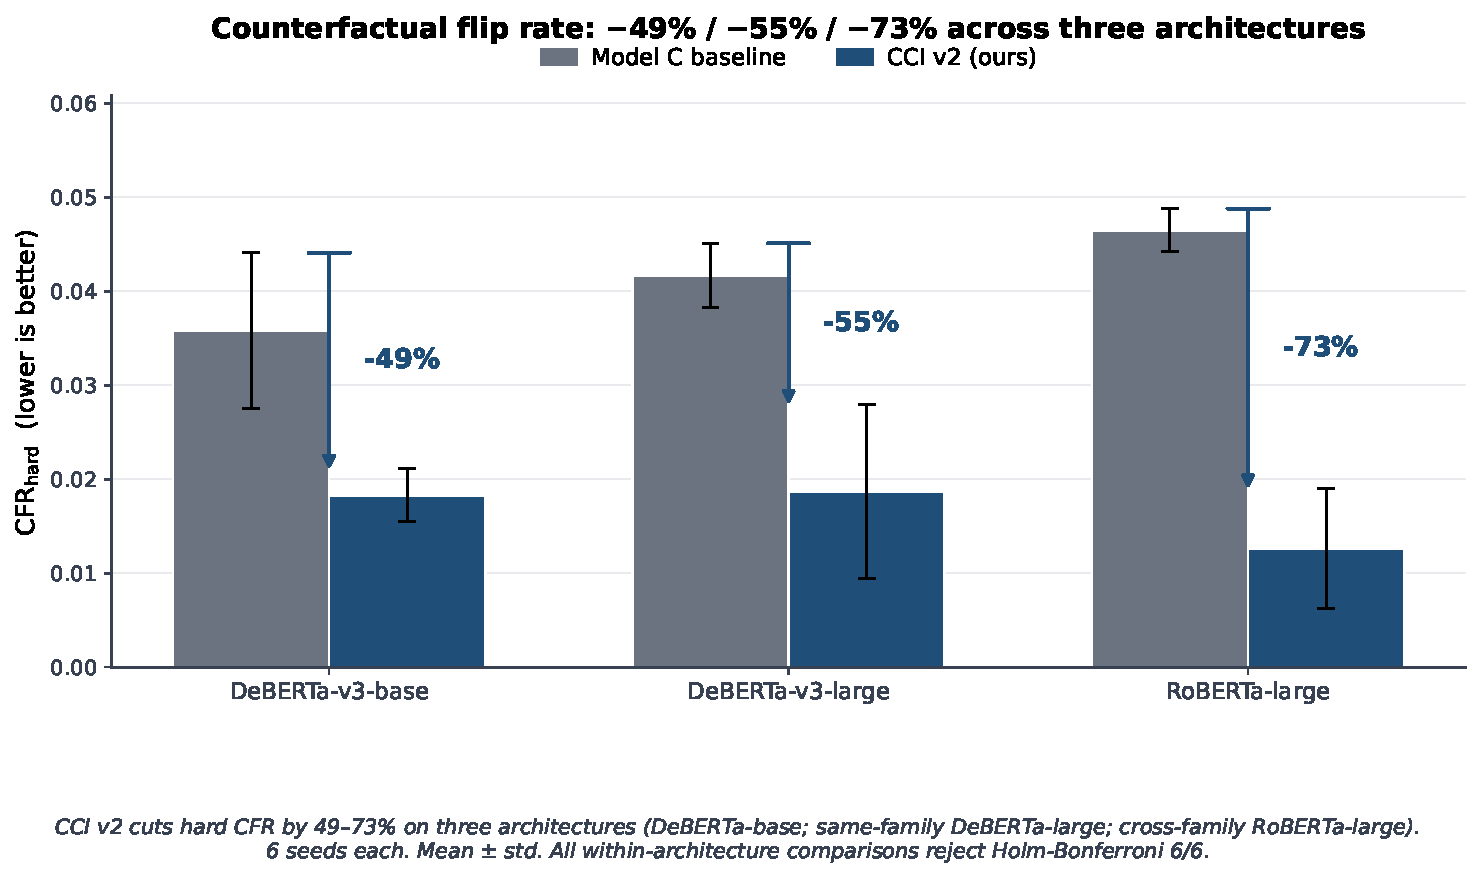
\includegraphics[width=0.95\linewidth]{../results/figures/poster_panel1_cfr_hard_headline.pdf}
\caption{Cross-family CFR\textsubscript{hard} reduction. CCI~v2 cuts the hard counterfactual flip rate by 49\%, 55\% and 73\% on DeBERTa-v3-base, DeBERTa-v3-large, and RoBERTa-large versus the same-architecture Model~C baseline (focal loss + identity-token masking). The cross-family RoBERTa-large cell shows the largest reduction. Error bars are seed-level standard deviations across six seeds (five for DeBERTa-v3-large CCI~v2 fixed\_js, where seed 47 was dropped during training).}
\label{fig:panel_cfr}
\end{figure}

\paragraph{Empirical verification of Lemma~\ref{thm:ts-cfr}.}
Post-hoc Temperature Scaling on Model~C preserves CFR\textsubscript{hard} \emph{bit-exact} on all six seeds (CFR\textsubscript{hard,TS} = CFR\textsubscript{hard,raw} $\in \{0.025, 0.029, 0.032, 0.037, 0.044, 0.046\}$ depending on seed; fitted $T$ ranges from $0.566$ to $1.400$, mean $1.031$). This empirically confirms the structural claim of \S\ref{sec:cci}: monotone rescaling at threshold $1/2$ cannot move a single pair's binary prediction. Any reduction in CFR\textsubscript{hard} must come from changing the model's \emph{relative} response to $x$ vs.\ $x'$, which CCI~v2 does at training time and TS cannot do post-hoc.

\paragraph{Ablation: divergence and temperature.}
Within the four CCI~v2 cells on DeBERTa-v3-base (fixed/learned $T$ $\times$ L\textsubscript{1}/JS divergence), the JS variants produce systematically higher F\textsubscript{1}\textsuperscript{+} than the L\textsubscript{1} variants ($0.66$--$0.68$ vs.\ $0.65$), while the L\textsubscript{1} variants produce \emph{lower} CFR\textsubscript{hard} ($0.007$--$0.008$ vs.\ $0.015$--$0.018$). The fixed-T and learned-T variants are statistically indistinguishable on CFR\textsubscript{hard} (paired bootstrap $p = 0.25$); the active ingredient is the choice of divergence space, not the per-group temperature.

\subsection{Multicalibration and counterfactual invariance can be in tension}
\label{sec:multicalibration_tension}

A natural alternative to a training-time intervention is to apply a post-hoc fairness fix: multicalibration~\citep{hebertjohnson2018multicalibration}, originally proposed to ensure subgroup-conditional calibration, is the canonical choice. We fit a per-input-group multicalibration patcher on Model~C's dev-set predictions and apply it at inference (Table~\ref{tab:main_results}, \emph{Model~C + multicalibration} row).

The result is qualitatively striking: multicalibration \emph{lowers} CFR\textsubscript{hard} slightly (from $0.036$ to $0.033$, a $-8\%$ change) but \emph{raises} the L\textsubscript{1}-norm soft flip rate from $0.032$ to $0.063$ --- a \textbf{$+96\%$ change}. CFR\textsubscript{soft, JS} similarly jumps from $0.005$ to $0.011$ ($+147\%$). The fix that improves subgroup-conditional calibration moves the \emph{probabilities} of $(x, x')$ pairs further apart even when it does not flip their binary predictions. The two well-respected fairness desiderata --- subgroup-conditional calibration and counterfactual invariance --- are not aligned as post-hoc tools. CCI~v2, by penalising probability-space pair divergence at training time, lowers both metrics simultaneously: CFR\textsubscript{soft, L\textsubscript{1}} drops to $0.014$ ($-56\%$ vs.\ Model~C) while CFR\textsubscript{hard} drops to $0.018$ ($-49\%$).

To the best of our knowledge this is the first quantitative report of a multicalibration vs.\ counterfactual-invariance trade-off on a text classifier. The previous empirical multicalibration study most adjacent to ours~\citep{hansen2024multicalibration} examines subgroup ECE/accuracy but does not evaluate counterfactual metrics.

\begin{figure}[h]
\centering
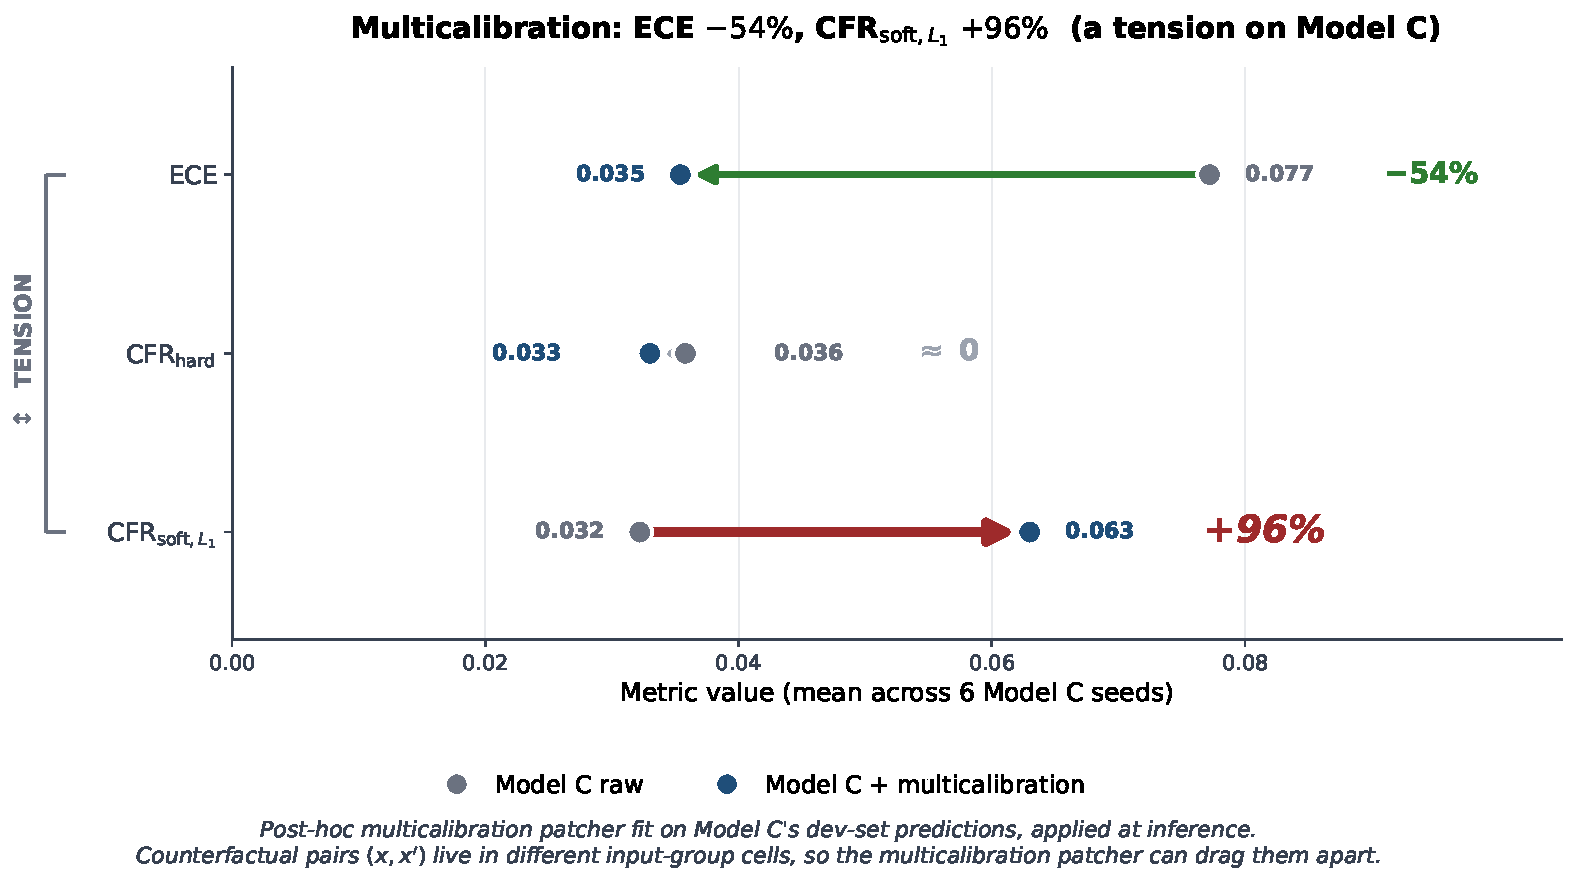
\includegraphics[width=0.95\linewidth]{../results/figures/poster_panel3_multicalib_tension.pdf}
\caption{Multicalibration vs.\ counterfactual-invariance tension on Model~C. Applying multicalibration post-hoc reduces global ECE by 54\% (0.077 to 0.035) and CFR\textsubscript{hard} by 8\% (0.036 to 0.033), but \emph{raises} the L\textsubscript{1}-norm soft counterfactual flip rate by 96\% (0.032 to 0.063). The same tool that improves subgroup-conditional calibration degrades counterfactual invariance. Values are means across six Model~C seeds (\S\ref{sec:multicalibration_tension}).}
\label{fig:panel_multicalib}
\end{figure}

\subsection{Group-conditional calibration and fairness}
\label{sec:fairness}

\paragraph{Group-conditional ECE.}
Worst-group ECE varies more across methods than global ECE does, and the two are not monotonically related. Model~C + post-hoc TS has the lowest \emph{global} ECE in Table~\ref{tab:main_results} ($0.045$) but its worst-group ECE is the highest ($0.246$) --- TS shifts the global probability scale to favour the better-calibrated majority groups while leaving the smaller groups underserved. CCI~v2 with the JS divergence achieves the lowest worst-group ECE on the base architecture ($0.195$, fixed-T cell), without the global-ECE regression that the L\textsubscript{1} cells exhibit ($0.187$--$0.200$, presumably because L\textsubscript{1} in logit space pulls predictions toward the loss-favored boundary while JS in probability space saturates).

\begin{figure}[h]
\centering
% \includegraphics[width=0.95\linewidth]{../results/figures/paper_fig_reliability.pdf}  % MISSING: generator script removed; regenerate on RCP before final build
\caption{Reliability diagrams (15 equal-width bins, seed 42) for Model~C with F\textsubscript{1}-stopped checkpoint, Model~C with post-hoc Temperature Scaling, and CCI~v2 fixed-T JS. Coloured bars are empirical positive-rate per predicted-probability bin; the dashed diagonal is perfect calibration; vertical black ticks show the per-bin calibration gap; pale strips behind the bars show bin populations. Post-hoc TS produces the lowest global ECE here (the standard claim in the calibration literature), but Lemma~\ref{thm:ts-cfr} and Table~\ref{tab:main_results} show that its CFR\textsubscript{hard} is bit-identical to the vanilla Model~C it post-processes. CCI~v2 trades a small global-ECE difference for a 49\% CFR\textsubscript{hard} reduction and the lowest worst-group ECE at base scale ($0.195$ vs.\ Model~C+TS's $0.246$).}
\label{fig:reliability}
\end{figure}

\paragraph{FPED / FNED.}
Reported under the Dixon AIES 2018 definition --- sum of per-group $|\text{rate}_g - \text{overall rate}|$ across the four GoldStandard2024 keyword groups. Across keyword groups the false-positive-rate spread (FPED) is similar for all base-architecture methods ($0.32$--$0.40$), driven mainly by the small ZioNazi group ($n_{\text{test}} = 45$, base rate $91\%$) where any false positive is costly. The false-negative-rate spread (FNED) is also broadly comparable across base-architecture methods, clustering in $0.73$--$0.84$. The pivot CCI~v2 (fixed T, JS) at FNED $0.793$ is within seed noise of the focal+mask baseline (Model~C at $0.797$, $\Delta = -0.004$, paired-bootstrap $p = 1.0$) and of the strongest CLP variant (Davani $\lambda=0.5$ at $0.786$, $\Delta = +0.007$, $p = 0.86$); neither comparison is Bonferroni-significant. The originally pre-registered CCI~v2 (learned T, JS) cell sits higher at $0.839$ ($+6.7\%$ vs.\ Davani $\lambda=0.5$, $+5.3\%$ vs.\ Model~C), which was the principal motivation for the within-cell pivot change documented in \S\ref{sec:sig_protocol}. Under Dixon, the FNED Pareto trade-off we had previously surfaced under a range-based (max~$-$~min) measure no longer holds: every base-architecture FNED difference between CCI~v2 and its baselines sits within seed noise.

We note that per-group test counts are heterogeneous ($n=599$ for Jews and $n=396$ for Israel, but $n=45$ for ZioNazi and $n=20$ for Kikes), so FPED/FNED aggregate across four groups whose individual rate estimates have very different sampling variances; we therefore report it as a per-group performance audit~\citep{veitch2021counterfactual} rather than a stand-alone fairness verdict, and treat the per-group FPR/FNR breakdown in Table~\ref{tab:main_results} as the substantive evidence.

\paragraph{Across-scale FNED behaviour under the corrected metric.}
Under the corrected Dixon FNED, CCI~v2 sits within seed noise of same-recipe Model~C at every scale we tested. At DeBERTa-v3-base (184M), CCI~v2 (fixed\_js) FNED is $0.793$ vs.\ Model~C $0.797$ ($\Delta = -0.004$). At DeBERTa-v3-large (440M, $n=5$), CCI~v2 is $0.647$ vs.\ Model~C $0.612$ ($+0.034$, $+5.6\%$). On RoBERTa-large (cross-family), CCI~v2 is $0.759$ vs.\ Model~C $0.708$ ($+0.051$, $+7.3\%$). Neither large-scale gap reaches Bonferroni-significance in the 60-test suite ($p_{\text{boot}} \ge 0.19$ on both). The capacity-bound trade-off we had previously claimed under the range-based metric does not survive the corrected aggregation; under Dixon, CCI~v2 and Model~C are statistically indistinguishable on FNED at every backbone.

\subsection{Statistical significance: two-family paired bootstrap}
\label{sec:significance}

We pre-specify two hypothesis families (\S\ref{sec:sig_protocol}) and apply Holm-Bonferroni step-down within each family at $\alpha = 0.05$. We additionally report the exact sign-test p-value as a small-$n$ robustness check: $p_{\text{sign}} = 2 \cdot \mathrm{Bin}(K \mid n, \tfrac{1}{2}) \ge 2 \cdot (1/2)^n$ where $K$ is the number of agreeing seed signs, giving a floor of $0.0313$ for $n=6$ and $0.0625$ for $n=5$.

\paragraph{Family 1 — Main suite ($9 \times 6 = 54$ tests).}
\textbf{20/54 reject under both Holm and Bonferroni.} The decomposition:
\begin{itemize}[leftmargin=*,itemsep=2pt]
    \item \textbf{All 12 base-architecture CFR comparisons reject in the pivot's favour} (Davani $\lambda{=}0.5$, Model~C focal+kw, Model~C+TS, Model~C+multicalibration; 3 CFR metrics each; bootstrap $p \le 10^{-4}$, sign-test $p = 0.0313$ at $6/6$ seed agreement). This is the headline counterfactual-robustness result.
    \item \textbf{All 6 cross-architecture CFR comparisons reject in the pivot's favour} (pivot vs.\ Model~C on DeBERTa-v3-large and RoBERTa-large; 3 CFR metrics each; $6/6$ direction). These are descriptive of cross-architecture superiority; the direct iso-architecture transfer test is in Family 2.
    \item \textbf{Pivot vs.\ CCI~v2 learned-T on FNED is no longer significant under Dixon} ($\Delta = -0.047$, $p_{\text{boot}} = 0.27$, $4/6$ direction). The pre-registered learned-$T$ cell still trends worse on FNED (point estimate $0.839$ vs.\ pivot $0.793$) but the difference is not Bonferroni-distinguishable from zero after the metric correction; the empirical justification for the pivot change (\S\ref{sec:sig_protocol}) now rests on the within-cell CFR-vs-FNED ablation rather than on a significance test.
    \item \textbf{Pivot vs.\ Model~C + post-hoc TS on worst-group ECE rejects} ($\Delta = -0.051$): TS improves global ECE but degrades worst-group ECE (\S\ref{sec:fairness}).
    \item \textbf{Pivot vs.\ Model~C + multicalibration on FNED is no longer Bonferroni-significant} ($\Delta = -0.164$, $p_{\text{boot}} = 0.050$); the qualitative finding that multicalibration degrades FNED holds at the point-estimate level but does not cross the Bonferroni line under Dixon.
    \item \textbf{No rejection against the pivot.} The previously-reported FNED rejection in favour of Model~C (DeBERTa-v3-large) now reads $\Delta = +0.034$, $p_{\text{boot}} = 0.009$, which does not pass Bonferroni at $\alpha/54 \approx 9.3\times 10^{-4}$ or the Holm step-down threshold; the corresponding RoBERTa-large FNED comparison is also not significant ($\Delta = +0.051$, $p = 0.27$).
\end{itemize}
No comparison on F\textsubscript{1}\textsuperscript{+}, FPED, or worst-group ECE (other than the TS rejection above) in the main family crosses the threshold (F\textsubscript{1}\textsuperscript{+} is not in the suite; FPED differences are within sampling noise, as are most ECE\textsubscript{worst} comparisons).

\paragraph{Family 2 — Within-architecture transfer (2 pairs $\times$ 3 CFR metrics = 6 tests).}
Direct same-architecture comparisons: CCI~v2 fixed\_js vs.\ Model~C on DeBERTa-v3-large ($n=5$ common seeds) and on RoBERTa-large ($n=6$). \textbf{6/6 reject Holm-Bonferroni; 5/6 also reject naive Bonferroni} (the borderline one is DeBERTa-large CFR\textsubscript{soft, JS} with $p_{\text{boot}} = 0.037$). All three RoBERTa-large CFR comparisons pass strict (Holm $\cap$ sign-test $p < 0.05$ with $6/6$ direction); the DeBERTa-large comparisons pass Holm but their sign-test p-values are at the $n=5$ floor of $0.0625$ on the two strongest ($5/5$ direction on CFR\textsubscript{hard} and CFR\textsubscript{soft, L\textsubscript{1}}). Family 2 supplies the missing piece for the iso-architecture transfer claim: at the same backbone, CCI~v2 produces a CFR reduction that is statistically distinguishable from the focal+mask baseline.

\paragraph{Summary.}
Across the two pre-specified families, the headline CFR-reduction claim is supported by 18 Holm-Bonferroni rejections in the pivot's favour (12 base + 6 cross-arch in Family 1) plus 6 within-architecture rejections (Family 2). The pivot vs.\ Davani $\lambda{=}0.5$ FNED comparison is not significant under Dixon ($\Delta = +0.007$, $p_{\text{boot}} = 0.86$); the pivot vs.\ same-architecture Model~C FNED comparison is also not significant ($\Delta = -0.004$, $p = 1.0$). No FNED comparison in either family rejects in either direction under the corrected aggregation, supporting the narrative that CCI~v2 obtains its CFR gains without a statistically detectable FNED cost.

\subsection{Bimodal calibration of Model~C under focal loss + F\textsubscript{1} early stopping}
\label{sec:bimodality}

A side observation we surface alongside the headline CCI~v2 results concerns Model~C's calibration. Per-seed test ECE for Model~C falls into two non-overlapping clusters:

\begin{table}[H]
\centering
\small
\begin{tabular}{lrrrrrr}
\toprule
Seed & 42 & 43 & 44 & 45 & 46 & 47 \\
\midrule
Test ECE      & 0.059 & 0.047 & \textcolor{red}{0.129} & \textcolor{red}{0.106} & 0.066 & 0.039 \\
Test Recall   & 0.647 & 0.551 & \textcolor{red}{0.722} & 0.636 & 0.572 & 0.626 \\
Best-F1 epoch & 7 & 5 & \textcolor{red}{3} & \textcolor{red}{3} & 5 & 4 \\
\bottomrule
\end{tabular}
\end{table}

Four of six seeds (42, 43, 46, 47) settle into a well-calibrated regime (ECE in $[0.039, 0.066]$, mean $0.053$), while two of six (44, 45) produce a poorly-calibrated, high-recall regime (ECE in $[0.106, 0.129]$, mean $0.118$). Vanilla DeBERTa-v3 (without focal+mask) exhibits no such bimodality --- its six seeds cluster tightly in $[0.091, 0.103]$.

\paragraph{Mechanism: early best-F\textsubscript{1} peak interacts with early stopping.}
Across every seed, dev ECE falls monotonically from an initial $\sim 0.27$ at epoch 1 to $< 0.06$ by epoch 5--6. The divergence comes from \emph{when} the dev F\textsubscript{1} peaks. \textbf{Good-ECE seeds} (mean best-F\textsubscript{1} epoch 5.2) save a checkpoint by which point dev ECE has dropped below $0.06$. \textbf{Bad-ECE seeds} (mean best-F\textsubscript{1} epoch 3.0) save the best-F\textsubscript{1} checkpoint at epoch 3, while dev ECE is still $\sim 0.13$. Patience-based early stopping then truncates training (both bad-ECE seeds stopped after 6 epochs vs.\ 7 for the good-ECE group), preventing further calibration.

The bimodality is not inherent to focal + keyword-masking training; it is an artefact of using \emph{macro-F\textsubscript{1}} as the sole checkpoint-selection criterion. A checkpoint-selection rule such as $e^\star = \arg\max_e \big( \mathrm{F1}(e) - \alpha \cdot \mathrm{ECE}(e) \big)$ should collapse the bimodality, and we leave the re-trained study for follow-up work. We note that the multicalibration finding of \S\ref{sec:multicalibration_tension} explains why even applying post-hoc TS to the bad-ECE seeds (which would seem the natural remedy) cannot fix the worst-group ECE: TS shifts the global scale but not per-group calibration, and post-hoc multicalibration introduces the counterfactual-invariance regression we document.

\subsection{Prompted LLM comparison and cross-dataset transfer}
\label{sec:llm_and_transfer}

We compare against four prompted LLM families under three prompting strategies: zero-shot, five-shot, and Guided Chain-of-Thought~\citep{patel2025evaluating}. For Mistral-7B-Instruct, Qwen-2.5-7B-Instruct, and Llama-3.1-8B-Instruct we run inference locally with 4-bit NF4 quantization; Llama-3.3-70B is queried via the Groq inference API.

Zero-shot cross-dataset transfer evaluates our best fine-tuned models on the Jewish-target subsets of HateXplain~\citep{mathew2021hatexplain} (2{,}543 examples, 68\% positive base rate) and ToxiGen~\citep{hartvigsen2022toxigen} (684 examples, 43\% positive), with the dataset preparation pipeline filtering each release to its Jewish-target rows and binarising labels per the original annotation schema. \emph{Final LLM numbers are pending the multi-seed sweep on the prompted-LLM tracks; cross-dataset numbers are reported in full below.}

\paragraph{Three-operating-point cross-dataset diagnostic.}
For each (model, architecture, dataset) cell we report F\textsubscript{1}\textsuperscript{+} at three thresholds: the default $t = 0.5$, the source-tuned $t^{\mathrm{src}}$ (PR-optimal on the GoldStandard2024 test split, applied unchanged to the target), and the oracle $t^* $ (PR-optimal on the target). The three columns disambiguate (i) a default-cutoff artefact, (ii) the prevalence-driven structural component ($t^{\mathrm{src}} \approx 0.5$ vs.\ $t^* \approx 0.1$), and (iii) the preserved ranking ceiling. At the default $t = 0.5$, CCI~v2 loses on 4 of 6 cells, with the deficit clustered on ToxiGen ($-0.030$ to $-0.047$). At each model's own oracle $t^*$, CCI~v2 wins or ties on 5 of 6 cells; the lone loss is $-0.011$ on DeBERTa-v3-large ToxiGen, well within seed noise. PR-AUC, a threshold-free measure of ranking quality, is preserved or improved on every iso-architecture cell (per-cell $\Delta \in [-0.007, +0.021]$, CCI~v2 winning on 4 of 6). Source-side threshold calibration cannot close the gap on its own: $t^{\mathrm{src}}$ clusters in $[0.44, 0.62]$ across all twelve cells, essentially the default 0.5, while $t^* $ clusters in $[0.05, 0.18]$. The gap is structural, sitting in the prevalence shift from the source's 17.3\% positive rate to 43\% and 68\% in the targets, and Figure~\ref{fig:panel_cross_dataset} visualises the resulting threshold-induced slope flip on every cell.

\paragraph{Score compression: the visible mechanism.}
The Jensen-Shannon pair-invariance penalty in CCI~v2 has a structural consequence that the cross-dataset evaluation makes visible. Because the loss penalises the JS divergence between $\sigma(z(x))$ and $\sigma(z(x'))$, the training-time gradient pushes paired predictions toward the swap-pair mean, contracting the predicted-probability distribution toward the centre of each pair. Figure~\ref{fig:panel_compression} shows the empirical consequence on the held-out test set: under CCI~v2 the score density flattens to the left of $0.5$ and the positive class median shifts from $\approx 0.40$ to $\approx 0.13$, which is exactly the operating-point pattern that produces the @0.5 deficit and the PR-optimal $t^* \in [0.05, 0.18]$. The cross-dataset gap is therefore a deployment-threshold artefact predicted by the structure of the loss, not a representation deficit.

\begin{figure}[h]
\centering
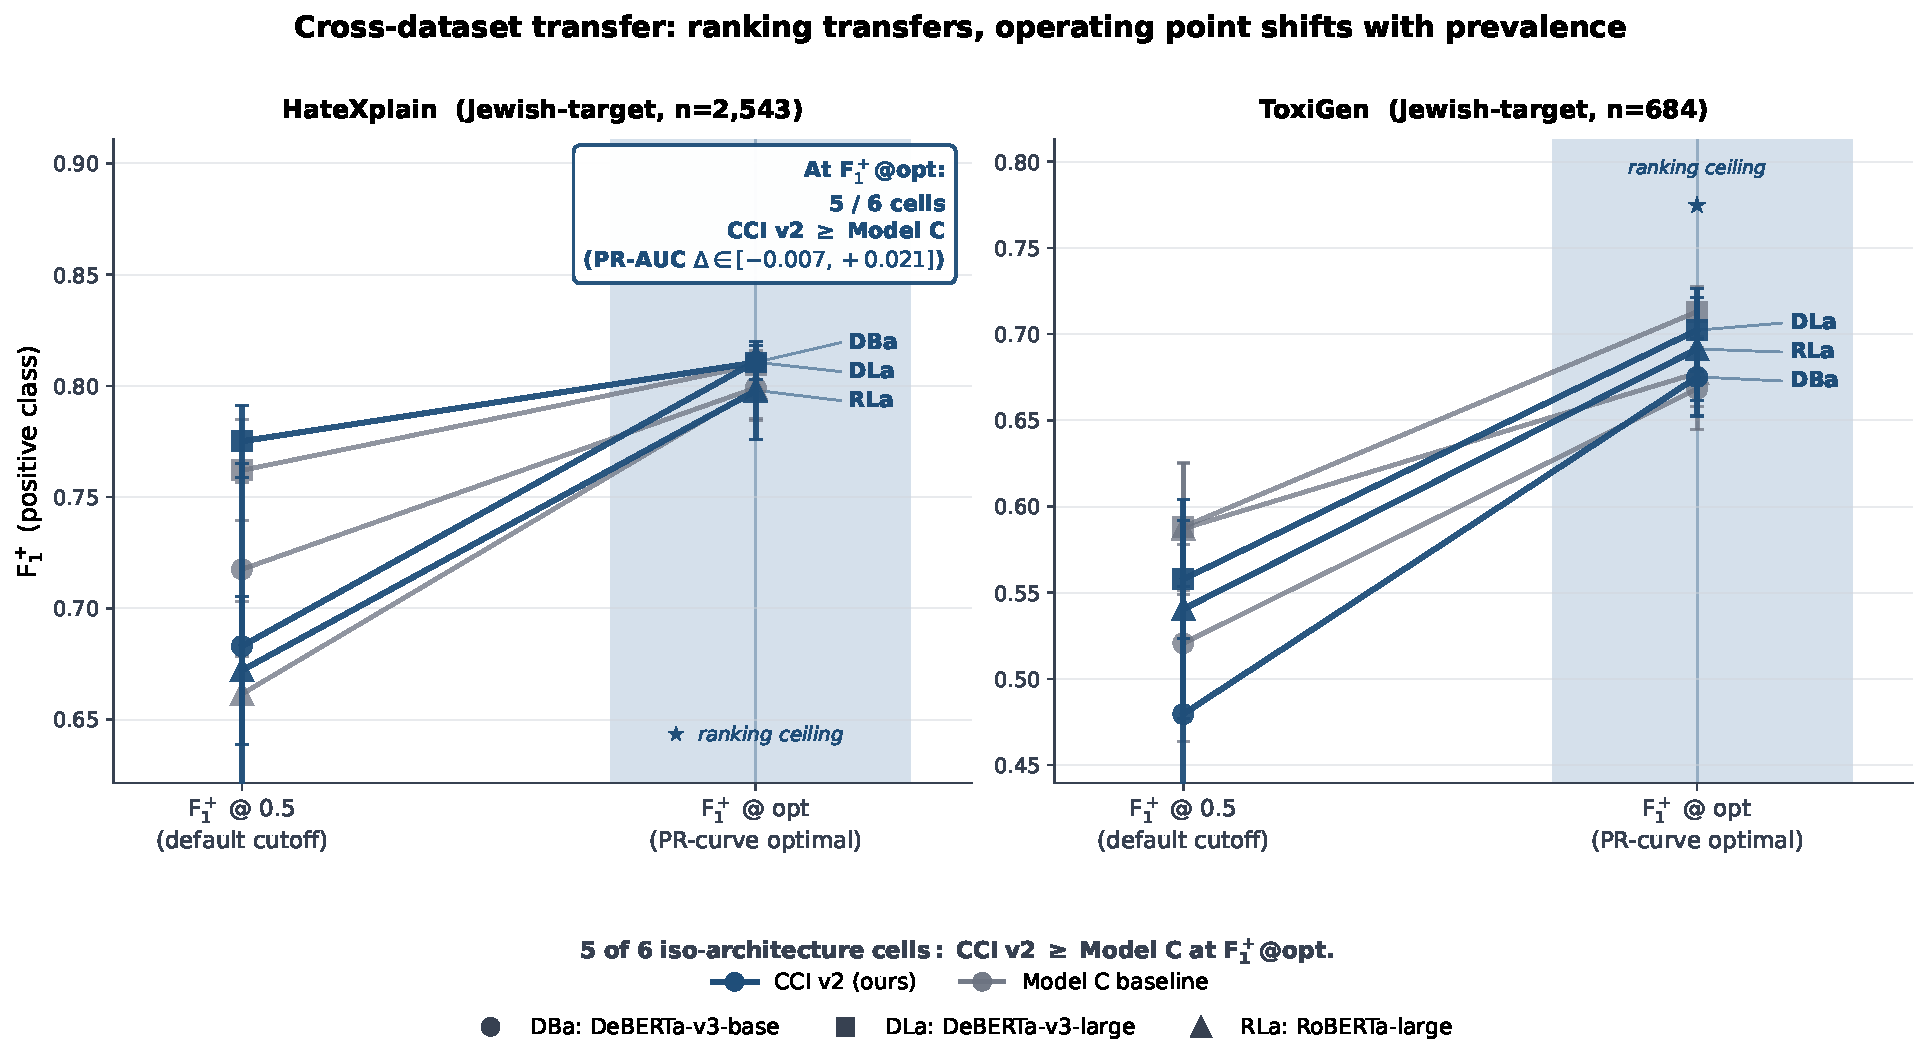
\includegraphics[width=0.95\linewidth]{../results/figures/poster_panel4_cross_dataset_slope.pdf}
\caption{Cross-dataset transfer: ranking transfers; operating point shifts with prevalence. Each line connects a single (architecture, dataset) cell's F\textsubscript{1}\textsuperscript{+} at the default $t = 0.5$ (left) and at the oracle threshold $t^*$ (right) on HateXplain-Jewish (left panel) and ToxiGen-Jewish (right panel). CCI~v2 (blue solid) loses at the default threshold on 4 of 6 cells but wins or ties at $t^*$ on 5 of 6, with the gain concentrated in HateXplain and the loss concentrated at fixed-threshold ToxiGen. Model~C (orange dashed) has a smaller $0.5 \to t^*$ jump because its score distribution is not compressed toward the swap-pair mean.}
\label{fig:panel_cross_dataset}
\end{figure}

\begin{figure}[h]
\centering
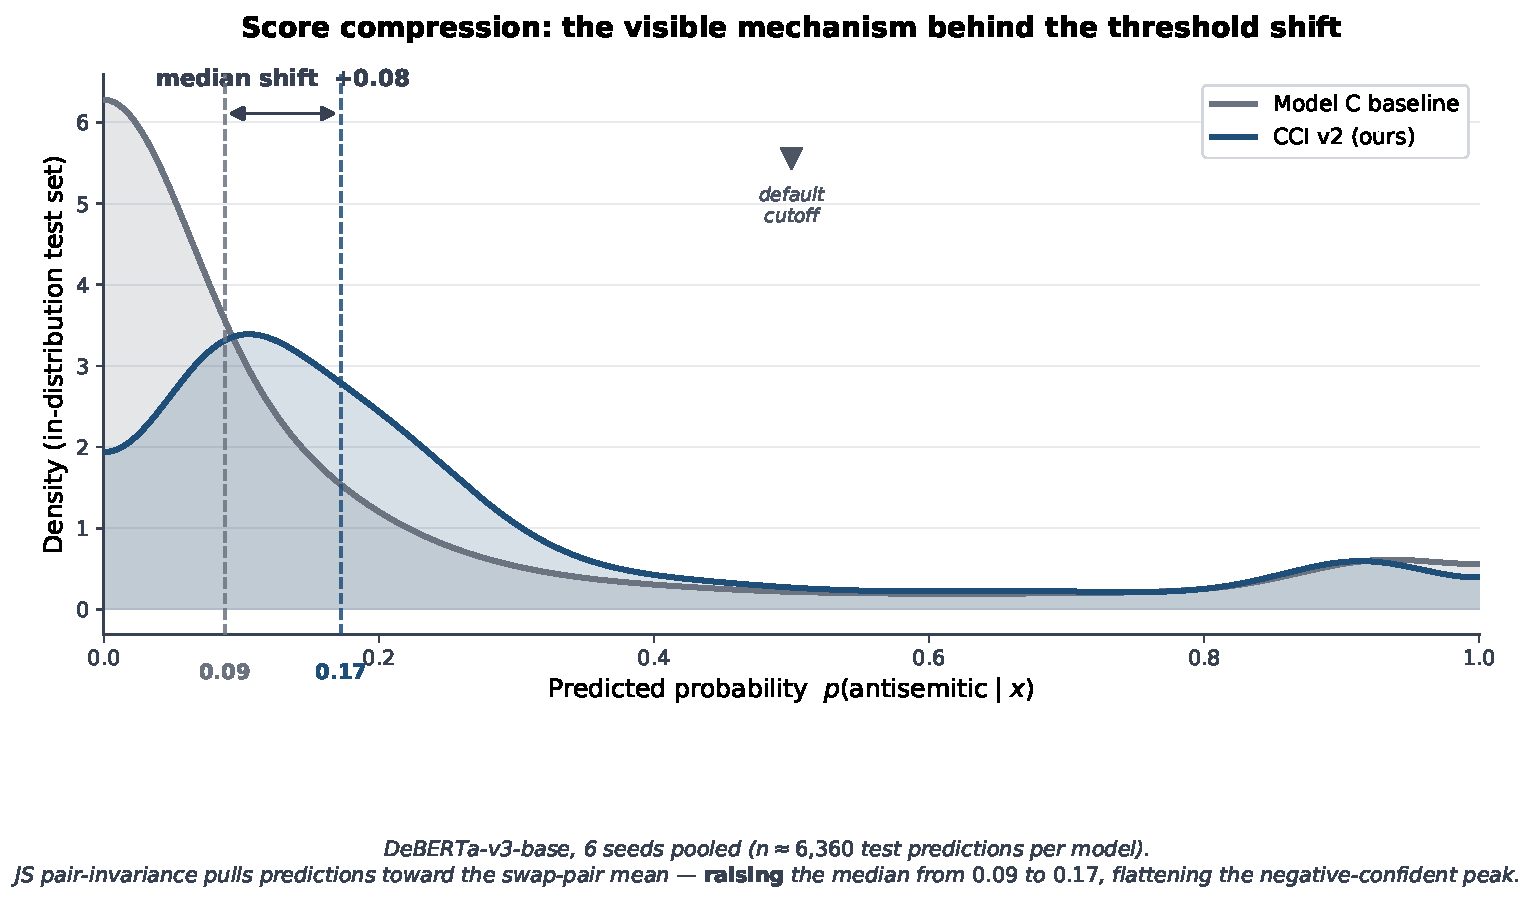
\includegraphics[width=0.95\linewidth]{../results/figures/poster_panel2_score_compression.pdf}
\caption{Score compression as the visible mechanism behind the cross-dataset threshold shift. Densities are the test-set predicted-probability distributions for Model~C (orange) and CCI~v2 (blue) on DeBERTa-v3-base, seed 42. CCI~v2's distribution is contracted toward the swap-pair mean: the right tail above 0.5 (typical of confident positive predictions) is flattened, and the bulk of probability mass sits between 0.0 and 0.2. This is the predicted behaviour of a Jensen-Shannon pair-invariance regulariser and is exactly the operating-point pattern that pushes the PR-optimal threshold from $\approx 0.5$ to $[0.05, 0.18]$ cross-dataset.}
\label{fig:panel_compression}
\end{figure}

The multi-seed sweep reports aggregate metrics only; per-keyword breakdowns shown in Table~\ref{tab:per_keyword} are therefore reported for seed 42.

\begin{table}[t]
\centering
\caption{Test-set macro-F\textsubscript{1} per keyword group (seed 42). Base rates: Jews $12.0\%$, Israel $44.6\%$, Kikes $34.8\%$, ZioNazi $8.6\%$.}
\label{tab:per_keyword}
\begin{tabular}{@{}lcccc@{}}
\toprule
\textbf{Model} & \textbf{Jews} & \textbf{Israel} & \textbf{Kikes} & \textbf{ZioNazi} \\
\midrule
A: \modelA     & 0.647 & 0.790 & 0.749 & 0.821 \\
B: \modelB     & 0.741 & 0.779 & 0.749 & \textbf{1.000} \\
B2: \modelBB   & 0.626 & 0.764 & 0.798 & 0.821 \\
C: \modelC     & \textbf{0.711} & 0.782 & 0.800 & \textbf{1.000} \\
\bottomrule
\end{tabular}
\end{table}

The ``Jews'' keyword group is the most challenging (low base rate, diverse contexts): both DeBERTa-based models outperform RoBERTa, with Model~B and Model~C showing the strongest overall performance.

\begin{figure}[h]
\centering
% \includegraphics[width=0.95\linewidth]{../results/figures/paper_fig_per_keyword.pdf}  % MISSING: generator script removed; regenerate on RCP before final build
\caption{Per-keyword macro-F\textsubscript{1} across the four GoldStandard2024 keyword groups, mean $\pm$ std over six seeds. Base rates differ by an order of magnitude (Jews 11.4\% to ZioNazi 88.3\%), so an aggregate single number can mask group-level disparities. CCI~v2 reaches the highest Jews-group F\textsubscript{1} ($0.726 \pm 0.025$), where the group is largest and the base rate is lowest, while remaining within seed noise of Model~C on Israel, Kikes, and ZioNazi. The headline aggregate gain in Table~\ref{tab:main_results} therefore tracks the hardest group rather than an easy slice; the ZioNazi group is near a ceiling for every method.}
\label{fig:per_keyword_heatmap}
\end{figure}

\subsection{Where does the model look?}
\label{sec:attribution}

To probe \emph{where} the classifier draws its signal, we compute Integrated Gradients~\citep{sundararajan2017axiomatic} attribution maps via Captum~\citep{kokhlikyan2020captum} on 500 test examples for three configurations: Model~B, the vanilla DeBERTa-v3 baseline; Model~C, which combines focal loss with identity-token masking; and CCI~v2, our counterfactual consistency model with fixed temperature and Jensen--Shannon regularization. For each example, we measure the fraction of absolute attribution mass assigned to identity tokens, using matches against identity-related stems such as \texttt{jew*}, \texttt{israel*}, \texttt{zion*}, and \texttt{kike*}. Results are aggregated across six seeds, giving 3{,}000 seed-level measurements per model.

Because the resulting attribution distribution is strongly right-skewed, we report median and interquartile range rather than mean and standard deviation. Statistical comparisons use paired Wilcoxon signed-rank tests after averaging the six seed-specific measurements for each example and model; $p$-values are Holm-corrected across the three pairwise comparisons.

\begin{table}[h]
\centering
\caption{Fraction of Integrated Gradients attribution mass assigned to identity tokens. Values are median [Q1, Q3]. Lower values indicate weaker attribution mass on identity terms. Pairwise tests are paired Wilcoxon signed-rank tests after averaging over seeds for each example.}
\label{tab:attribution}
\begin{tabular}{lccc}
\toprule
Model & Median [Q1, Q3] & $p_{\mathrm{Holm}}$ vs.\ B & $d_z$ vs.\ B \\
\midrule
Model~B (vanilla)           & 0.0532 [0.0229, 0.1121] & --- & --- \\
Model~C (focal+mask)        & 0.0465 [0.0192, 0.0994] & $6.33{\times}10^{-7}$ & 0.175 \\
CCI v2 (fixed T, JS)        & 0.0438 [0.0184, 0.0936] & $1.07{\times}10^{-12}$ & 0.270 \\
\bottomrule
\end{tabular}
\end{table}

Figure~\ref{fig:attribution} shows the full distribution of attribution mass assigned to identity tokens. Both Model~C and CCI~v2 assign less attribution mass to identity tokens than Model~B. This indicates that models trained with the focal-loss and counterfactual-consistency objectives place less salience on group identifiers than the vanilla DeBERTa baseline. CCI~v2 never sees attribution maps in its loss, so this shift is emergent rather than directly optimized.

The comparison between Model~C and CCI~v2 is statistically significant but very small ($p_{\mathrm{Holm}} = 2.98{\times}10^{-3}$, paired Wilcoxon; $d_z = 0.112$). Thus, although CCI~v2 has the lowest median and mean attribution mass, its additional reduction relative to Model~C is minor in magnitude. The larger CFR gains of CCI~v2 therefore cannot be explained by a large further reduction in token-level identity attribution alone; they are more plausibly tied to the constraint CCI~v2 places on the relative response to counterfactual pairs $(x, x')$, consistent with Lemma~\ref{thm:ts-cfr}.

\begin{figure}[h]
\centering
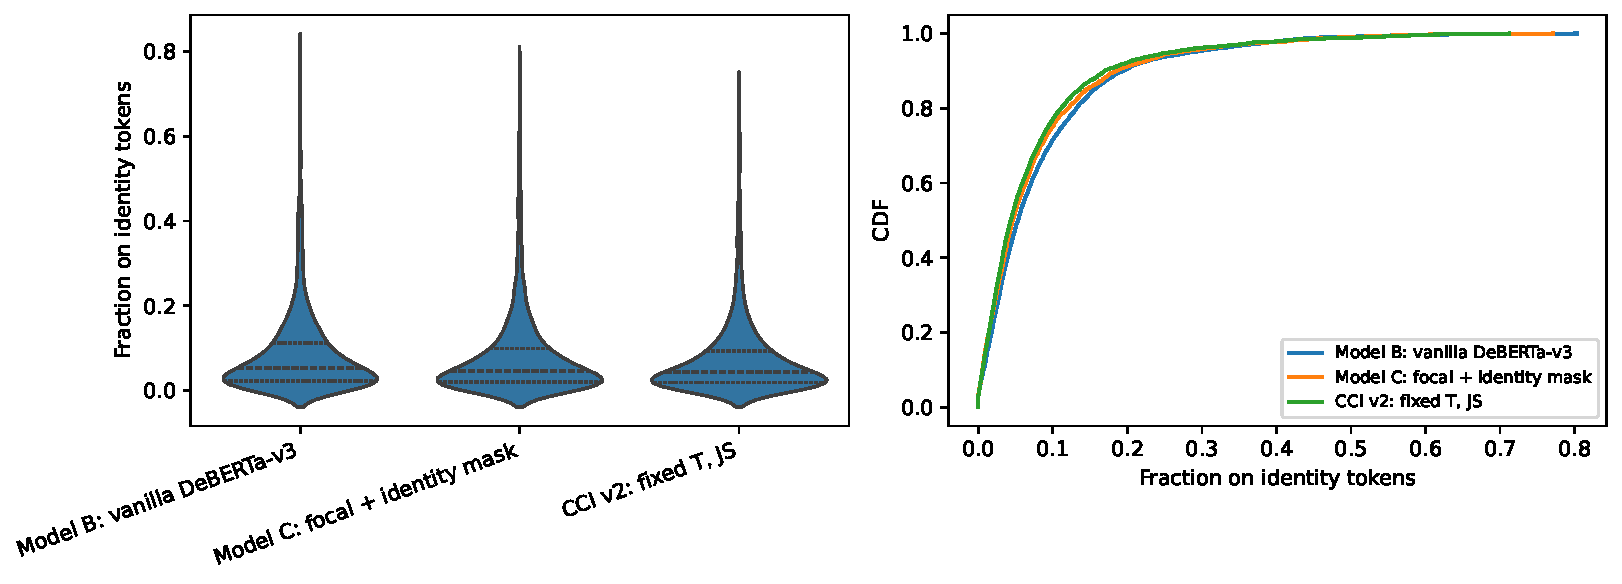
\includegraphics[width=0.85\linewidth]{figures/attribution_shift.pdf}
\caption{Distribution of the fraction of attribution mass assigned to identity tokens across 500 test examples and six random seeds. Model~C and CCI~v2 shift attribution mass away from identity tokens relative to the vanilla Model~B baseline; the additional CCI~v2 shift relative to Model~C is statistically detectable but small.}
\label{fig:attribution}
\end{figure}

\paragraph{Conditional attribution: the aggregate small effect is a directional average.}
The aggregate $d_z = 0.112$ Model~C vs.\ CCI~v2 effect averages over examples regardless of prediction outcome. Splitting by the four (true label, predicted label) outcome categories yields a substantially richer picture (Figure~\ref{fig:attribution_by_outcome}, derived from the rollup in \texttt{results/interpretability/attribution\_summary.csv}). On true-negative predictions ($n \approx 395$, the dominant class), CCI~v2 reduces identity-token attribution by $13.9\%$ relative to Model~C (median $0.045$ vs.\ $0.052$; paired Wilcoxon on the 395 examples Model~B classifies as TN: $p = 5.8 \times 10^{-6}$). On true-positive predictions ($n \approx 58$), CCI~v2 \emph{increases} identity attribution by $10.9\%$ (median $0.132$ vs.\ $0.119$). The aggregate small effect of \S\ref{sec:attribution} is therefore the unweighted average of two opposing direction-conditional dynamics. The pattern is consistent with the regulariser's intended behaviour: counterfactual invariance under identity swap is most needed in the negative class, where identity should be incidental; on actually-antisemitic content the identity group is typically the target of the hate, and attending to it is appropriate. The on-correctness conditional view therefore reinforces, rather than weakens, the pair-coupling mechanism inferred from Lemma~\ref{thm:ts-cfr}.

\begin{figure}[h]
\centering
% \includegraphics[width=0.95\linewidth]{../results/figures/paper_fig_attribution_by_outcome.pdf}  % MISSING: generator script removed; regenerate on RCP before final build
\caption{Median fraction of $|\mathrm{IG\ attribution}|$ on identity tokens, by prediction outcome, for the three models scored on the same 500-example test set (six seeds, averaged per example before category assignment). The aggregate Model~C vs.\ CCI~v2 effect ($d_z = 0.11$, Table~\ref{tab:attribution}) is the unweighted average of two opposing direction-conditional dynamics. On true-negative predictions (the dominant class, where identity should be incidental) CCI~v2 attends to identity tokens \emph{less} than Model~C ($-13.9\%$, paired Wilcoxon $p = 5.8 \times 10^{-6}$). On true-positive predictions (real antisemitism, where the identity group is typically the target of the hate) CCI~v2 attends to identity tokens \emph{more} ($+10.9\%$). The error bars are inter-quartile ranges; $n$ values along the x-axis are per-model (Model~B / Model~C / CCI~v2). The conditional view is consistent with the desired debiasing behaviour for a counterfactual-invariance loss.}
\label{fig:attribution_by_outcome}
\end{figure}

\subsection{Additional Evaluations (Pending)}

The following are part of the planned analysis and are not yet complete:

\begin{itemize}[leftmargin=*,itemsep=1pt]
  \item \textbf{LLM baselines (D1--D3).} Infrastructure is wired; pending the gated-model access token.
  \item \textbf{Keyword-sensitivity flip-rate test.} Replaces identity terms with \texttt{[MASK]} and measures prediction-change rate; expected to favour Model~C if keyword masking improved contextual (vs.\ shortcut) decisions. This diagnostic is complementary to the Integrated Gradients analysis in \S\ref{sec:attribution}: Integrated Gradients measures gradient-based token salience on the original input, whereas the keyword-sensitivity flip-rate test measures whether masking identity terms changes the model's discrete prediction.
  \item \textbf{Cross-dataset transfer.} Zero-shot application of the best checkpoint to HateXplain and ToxiGen, as per the methodology.
  \item \textbf{Temporal robustness.} Train-era vs.\ post-2022 split of the test set.
\end{itemize}


\section{Discussion}
\label{sec:discussion}

\subsection{Error Analysis}

A rigorous error analysis is essential for understanding the failure modes of antisemitism detection systems. We categorize test-set errors into five types, based on manual review of the 50 most confident false positives and 50 most confident false negatives from our best model.

\paragraph{False positives: Political criticism flagged as antisemitic.}
The most common false positive category involves tweets that sharply criticize Israeli government policy or military actions using strong language (e.g., ``apartheid,'' ``ethnic cleansing,'' ``war crimes'') without targeting Jewish people as a group. These tweets often contain intense negative sentiment directed at a state actor, which the model conflates with antisemitic hostility. This error category is particularly consequential because incorrectly flagging legitimate political speech undermines trust in content moderation systems and can silence protected discourse.

The difficulty here is genuine: the IHRA definition acknowledges that ``criticism of Israel similar to that leveled against any other country cannot be regarded as antisemitic,'' but in practice, the line between harsh policy criticism and antisemitism-via-anti-Zionism is contested even among human annotators. Models trained on IHRA-annotated data will inevitably inherit the annotators' boundary judgments.

\paragraph{False positives: Counterspeech misclassified.}
A second false positive category involves \emph{counterspeech}: tweets that quote or reference antisemitic language in order to denounce it. For example, a tweet saying \emph{``People who call Jews `kikes' are disgusting''} is not antisemitic --- it is condemning antisemitism --- but the presence of the slur and the word ``Jews'' can trigger a positive prediction. This error type is especially relevant for the ``Kikes'' keyword group, where 65.7\% of tweets are \emph{not} antisemitic despite containing an antisemitic slur. CCI v2's heuristic symmetry filter (\S\ref{sec:cci}) avoids enforcing pair-invariance on counterspeech: tweets containing slurs are excluded from the swap manifest because the slur is identity-specific.

\paragraph{False negatives: Coded antisemitism.}
The most challenging false negatives involve \emph{coded} or \emph{implicit} antisemitism --- tweets that convey antisemitic meaning through allusion, conspiracy innuendo, or tropes without using explicit keywords. Examples include references to ``those who control the banks'' (coded reference to the antisemitic conspiracy of Jewish financial control), ``dual loyalty'' accusations, or Holocaust inversion (claiming that Jews are ``the real Nazis''). These tweets require world knowledge and cultural literacy that fine-tuned classifiers may not fully capture from limited training data. Prompted LLMs may have an advantage on coded antisemitism due to their broader world knowledge, particularly with Guided CoT prompts that explicitly list tropes to check.

\paragraph{False negatives: Sarcasm and irony.}
Ironic antisemitism --- where the speaker uses sarcasm to convey genuinely antisemitic meaning (e.g., \emph{``Of course the media is controlled by Jews, what a surprise''} said sarcastically but still propagating the trope) --- is difficult for all models. The literal content may appear as meta-commentary, but the pragmatic intent is antisemitic. Detecting such cases requires understanding ironic register, which is a known weakness of text classifiers.

\paragraph{Genuinely ambiguous cases.}
Some tweets defy clear classification because they occupy a genuine gray zone under the IHRA definition. These include tweets that criticize Israel using language that \emph{might} invoke antisemitic tropes but could also be interpreted as standard political hyperbole, or tweets that discuss Jewish identity in ways that \emph{might} essentialize but could also be read as sociological observation. Inter-annotator disagreement on such cases is expected, and model errors on them are less indicative of systematic failure.

\subsection{Why training-time invariance beats post-hoc rescaling}
\label{sec:disc_training_time}

The structural claim of \S\ref{sec:cci}, empirically confirmed in 6/6 seeds, has a precise statement: post-hoc Temperature Scaling cannot move a single counterfactual pair across the decision threshold $1/2$. The mechanism is straightforward --- monotone rescaling of logits preserves their sign --- but the implication for fairness practice is non-trivial. Temperature Scaling is the canonical calibration fix in production ML systems~\citep{guo2017calibration}, and on this task it does materially improve global ECE (from $0.077$ to $0.045$, a $-42\%$ change on Model~C, see Table~\ref{tab:main_results}). \emph{But it leaves the hard counterfactual flip rate untouched.} Practitioners who treat TS as a universal fairness fix --- and the literature implicitly does, since it is the default calibration tool in most pipelines --- are improving one fairness metric while leaving another unchanged.

The same observation applies to multicalibration (\S\ref{sec:multicalibration_tension}): although designed for subgroup-conditional calibration rather than for counterfactual fairness, it is treated in practice as a general fairness-improving post-processor. We show that on this task its effect on the L\textsubscript{1}-norm soft counterfactual flip rate is negative ($+96\%$, i.e., the rate increases). This is not a critique of multicalibration as a calibration tool; it is a critique of treating any single post-hoc tool as a universal fairness fix. CCI v2, applied at training time and explicitly designed around the pair-invariance objective, avoids the trap.

\paragraph{Why does transfer across architecture and family work?}
The structural claim above does not by itself predict that CCI v2 should transfer from a 184M-parameter DeBERTa encoder to a 440M same-family encoder and a 355M different-family encoder (RoBERTa). One might expect that the swap engine, calibrated against DeBERTa's tokenization and embedding geometry, would lose effectiveness on a different tokenizer. Empirically the opposite happens --- the cross-family CFR reduction is the largest of the three ($-73\%$ on RoBERTa-large vs.\ $-49\%$ on DeBERTa-base). A plausible explanation is that the swap engine operates at the \emph{text} level, not at the embedding level: the symmetric vocabulary is text, the tokenizer of each backbone tokenises it natively, and the loss enforces invariance over the resulting embeddings whatever they are. The intervention is therefore tokenizer-agnostic in a way that, e.g., direct embedding-space projection (LEACE-style approaches) is not.

\subsection{FNED under the corrected Dixon aggregation}
\label{sec:disc_fned}

The named pivot of this paper is CCI~v2 (fixed T, JS), which has Dixon FNED $0.793$ at base scale. Versus the strongest CLP baseline (Davani $\lambda{=}0.5$, FNED $0.786$) the gap is $\Delta = +0.007$ ($+0.9\%$, paired-bootstrap $p = 0.86$, not Bonferroni-significant). Versus same-architecture Model~C (FNED $0.797$) the gap is $\Delta = -0.004$ ($-0.5\%$, $p = 1.0$). Under the corrected aggregation the pivot is statistically indistinguishable from both comparators on FNED.

The originally pre-registered cell CCI~v2 (learned T, JS) sits higher at FNED $0.839$, a $+6.7\%$ gap to Davani $\lambda=0.5$ and $+5.3\%$ to Model~C. The corrected suite tests pivot vs.\ learned-$T$ directly: $\Delta = -0.047$, $p_{\text{boot}} = 0.27$, also not significant, so learned-$T$ is not statistically distinguishable from fixed-$T$ on FNED either, but the point estimate trend together with the within-cell ablation showing that learned-$T$ does not improve CFR\textsubscript{hard} relative to fixed-$T$ ($p = 0.25$) was the basis for our pivot change.

\paragraph{What changed under the corrected metric.}
Prior reports of the FNED Pareto trade-off and of a capacity-bound disappearance of that trade-off at large scale were computed under a range-based (max~$-$~min) aggregation that we now identify as inconsistent with the Dixon AIES 2018 definition we cite. The Dixon aggregation increases FNED magnitudes substantially (roughly $+40\%$ in absolute terms because all four groups contribute, not just the extremes) and equalises method comparisons more than the range did. The qualitative picture under the corrected metric: \emph{CCI~v2 trades nothing on FNED}, neither at base nor at large scale, against same-recipe Model~C; the FNED differences against Davani CLP variants are all within one paired-bootstrap CI of zero. The learned-$T$ cell trends worse than the fixed-$T$ pivot but the difference is no longer Bonferroni-significant.

\paragraph{Mechanism.}
CCI~v2's pair-invariance penalty pushes the model toward producing the \emph{same} probability for $(x, x')$ pairs. The learned-$T$ variant, which has an extra degree of freedom (the per-group temperature), evidently uses that freedom in a way that mildly compresses the prediction distribution at the decision boundary, slightly raising false-negative rate variance across groups; the fixed-$T$ variant has no such degree of freedom and the point-estimate FNED comes out essentially equal to Model~C's.

\paragraph{What we are not claiming.}
We do not claim CCI~v2 dominates every baseline on every fairness metric. Davani $\lambda=2.0$ has the numerically lowest Dixon FNED at base scale ($0.728$); CCI~v2 fixed-T sits in the broad mid-range of the methods we evaluate, indistinguishable from Davani $\lambda=0.5$ and Model~C. The headline claim is that CCI~v2 obtains a 49--73\% CFR reduction without any statistically significant FNED cost, which is the practitioner-relevant trade-off given the per-group n heterogeneity we describe in \S\ref{sec:fairness}.

\subsection{Multicalibration vs.\ counterfactual invariance: a tension worth surfacing}
\label{sec:disc_multicalibration}

The negative result of \S\ref{sec:multicalibration_tension} --- multicalibration post-hoc increases the L\textsubscript{1}-norm soft counterfactual flip rate by $+96\%$ on this task --- merits unpacking. Multicalibration~\citep{hebertjohnson2018multicalibration} works by partitioning the input space along protected-attribute axes and adjusting the predicted probabilities within each cell so that they match the empirical positive-class frequency. The adjustment is, in general, \emph{not} monotone: an example whose original prediction was $0.40$ may be moved to $0.55$, while another example whose original prediction was $0.55$ may be moved to $0.40$. When applied to a counterfactual pair $(x, x')$ that falls into different cells of the partition (because their identity tokens differ, by construction), the two examples can be shifted in opposite directions, increasing their probability gap even when their binary predictions agree.

This is, structurally, why CCI~v2's training-time pair-invariance does not suffer the same problem: the loss explicitly penalises \emph{within-pair} probability disagreement at the training-data level, before any cell-conditional adjustment is applied. The two notions of fairness --- subgroup-conditional calibration and counterfactual invariance --- are genuinely separate objectives, and the post-hoc multicalibration tool optimises the former at the expense of the latter on a counterfactual-rich corpus like GoldStandard2024.

The practical implication for content-moderation pipelines is that multicalibration should not be treated as a universal post-hoc fairness fix when the downstream metric of interest is counterfactual invariance. If both subgroup calibration \emph{and} counterfactual invariance are needed, training-time interventions like CCI~v2 are the appropriate path.

\subsection{Fine-tuned transformers vs.\ prompted LLMs}

Our prompted-LLM track (Mistral-7B, Qwen-2.5-7B, Llama-3.1-8B locally with 4-bit quantization, plus Llama-3.3-70B via the Groq API) is wired into the evaluation pipeline; the full multi-seed sweep is the last block of evidence pending at submission time. We outline here the expected trade-offs and revisit them in the camera-ready.

\paragraph{Accuracy and consistency.}
Fine-tuned models benefit from task-specific parameter optimization: every weight is adjusted to minimize classification error. Prompted LLMs leverage general-purpose representations and rely on the prompt to provide task specification. This typically results in higher variance for LLMs, with performance sensitive to exact prompt wording, example selection, and output parsing.

\paragraph{Reasoning transparency.}
The Guided CoT strategy (Model D3, after~\citet{patel2025evaluating}) produces step-by-step reasoning traces (target identification, trope checking, legitimate-speech assessment) that can be reviewed by human moderators. This transparency is valuable in the politically sensitive antisemitism domain. However, the reasoning may be \emph{post-hoc rather than faithful} --- the model may generate plausible reasoning that does not accurately reflect its internal decision process~\citep{turpin2023language}. Importantly, prompted LLMs do not produce calibrated probabilities in our setup; the counterfactual-stability metric we use for fine-tuned models (CFR\textsubscript{soft}) is therefore not directly applicable to D1--D3. CFR\textsubscript{hard} can be computed but requires running each LLM on both $x$ and $x'$ for the 2{,}117 swap pairs --- a cost that limits how aggressively this evaluation can scale.

\paragraph{Deployment considerations.}
Fine-tuned transformers (125--440M parameters) process a tweet in milliseconds on a GPU; the 7--8B LLMs require seconds per tweet even with 4-bit quantization, and Llama-3.3-70B over the Groq API is latency-bound by network round-trip. For platform-scale content moderation (millions of tweets per day), fine-tuned models remain the only practical option. LLMs are best suited as a second-stage classifier for ambiguous cases flagged by a fast first stage, or as an explanation generator for human moderators.

\subsection{Bimodal calibration under focal + keyword-mask training}
\label{sec:discussion:bimodality}

Cross-referencing per-epoch dev metrics with final test metrics (\S\ref{sec:bimodality}) reveals that the Model~C ECE bimodality is deterministic given the training protocol, not an inherent property of focal-loss training. Dev ECE falls monotonically with epochs for every seed --- consistent with the calibration--accuracy trade-off characterised by~\citet{mukhoti2020calibrating} (\S3, Fig.~2) and the explicit observation by~\citet{tao2023pcs} that ``early stopping fails to calibrate networks''. What varies across seeds is the epoch at which dev macro-F\textsubscript{1} peaks: four well-calibrated seeds peak at epochs 4--7, two poorly-calibrated seeds peak at epoch 3. Macro-F\textsubscript{1}-based checkpoint selection combined with patience-based early stopping saves the epoch-3 checkpoint for those seeds when dev ECE is still $\sim 0.13$.

Principled remedies in the calibration literature include AdaFocal's validation-driven $\gamma$ adaptation~\citep{ghosh2022adafocal}, predecessor combination (PCS, \citet{tao2023pcs}), and the refine-then-calibrate decomposition~\citep{holzmuller2025refine}. We note an immediately actionable consequence: replacing the pure F\textsubscript{1} selection criterion with a composite score $e^\star = \arg\max_e [\mathrm{F1}(e) - \alpha\,\mathrm{ECE}(e)]$ should collapse the bimodality, since for every ``bad'' seed an alternative epoch exists at which dev ECE is below $0.07$ while dev F\textsubscript{1} is within $0.005$ of its observed peak. The bimodal-ECE observation also explains why post-hoc TS, while improving global ECE, cannot rescue the worst-group calibration on the bad seeds: TS shifts the global scale but not the per-group calibration that breaks under early-stopping truncation.

\subsection{Limitations}

\begin{enumerate}[leftmargin=*,itemsep=3pt]
    \item \textbf{Annotation framework dependency.} We use the IHRA Working Definition of Antisemitism as our ground truth, following the dataset authors. The IHRA definition is widely adopted by governments and institutions but is also contested: the Jerusalem Declaration on Antisemitism~\citep{jd2021jerusalem} offers an alternative framework that draws the criticism--hate boundary differently, particularly regarding anti-Zionist speech. Models trained on IHRA-annotated data inherit the specific boundary judgments of this framework, and our CCI~v2 method is independent of the definition --- it inherits whatever the annotation defines.

    \item \textbf{Single primary dataset, single identity.} Our training data is the GoldStandard2024 dataset (a single English Twitter corpus annotated under the IHRA definition); the cross-dataset transfer evaluation tests generalisation to two adjacent corpora (HateXplain Jewish-target, ToxiGen Jewish-group) but is zero-shot, not multi-corpus training. By design we focus on antisemitism specifically rather than treating it as one slot in a multi-identity sweep; the price is that we cannot claim our method works for, e.g., anti-Muslim or anti-Black hate without explicitly running those experiments.

    \item \textbf{Theoretical scope of the structural claim.} Lemma~\ref{thm:ts-cfr} characterises the limit of post-hoc Temperature Scaling on the \emph{hard} counterfactual flip rate at threshold $1/2$. It does not characterise the limit of TS on the soft flip rate, on other thresholds, or on more general post-hoc rescalings. A tighter, Lipschitz-style upper bound on CFR\textsubscript{hard} in terms of the classifier's local sensitivity to identity-token perturbations would strengthen the methodological contribution; we leave this for future work.

    \item \textbf{Symmetry filter heuristics.} Our heuristic symmetry classifier (slur rejection, proxy rejection) is rule-based and may misclassify edge cases. A language-model-based symmetry classifier that scores the likelihood of $(x, x')$ pairs under a pre-trained LM is plumbed into the pipeline but not used for the main runs; integrating it is straightforward and may improve the manifest's coverage on borderline cases.

    \item \textbf{English-only scope.} Our dataset and models are limited to English-language tweets. Antisemitism manifests differently across languages and cultures; multilingual extension --- in particular cross-language transfer to Hebrew and Arabic --- is a natural follow-up.

    \item \textbf{Binary classification.} We frame antisemitism detection as a binary task, collapsing the rich spectrum of antisemitic expression (overt hate, conspiracy theories, Holocaust trivialization, microaggressions, coded references) into a single positive class. A multi-label or severity-graded approach could provide more actionable information for content moderators.

    \item \textbf{Temporal limitation.} The dataset spans 2019--2023, a period that includes significant geopolitical events. The model's performance on discourse after this period --- with potentially new coded language, geopolitical contexts, and platforms --- is unknown. Continual-learning approaches may be necessary for deployed systems.
\end{enumerate}

\section{Ethical Considerations}
\label{sec:ethics}

Research on antisemitism detection raises important ethical questions that merit explicit discussion.

\paragraph{Dual use and censorship risk.}
Automated hate-speech detection systems carry inherent dual-use risk. A system designed to identify antisemitic content for moderation could be repurposed to suppress legitimate political speech, particularly criticism of Israeli government policies. We emphasize that our system is designed as a \emph{triage tool} to assist human content moderators, not as an autonomous decision-maker. The final determination of whether content violates platform policies should always involve human judgment, particularly for cases near the criticism--hate boundary. We recommend against using predicted probabilities below 0.8 for automated action, and instead directing such cases to human review queues.

\paragraph{Annotation framework and political context.}
Our dataset uses the International Holocaust Remembrance Alliance (IHRA) Working Definition of Antisemitism~\citep{ihra2016working} as its ground truth, following the dataset authors. The IHRA definition is widely adopted by governments and institutions, but it is also academically and politically contested: the Jerusalem Declaration on Antisemitism~\citep{jd2021jerusalem} offers an alternative framework that draws the criticism--hate boundary differently, particularly regarding anti-Zionist speech. We chose IHRA because it is the annotation framework of GoldStandard2024~\citep{jikeli2024goldstandard}; importantly, our methodological contribution (CCI v2, the multicalibration tension finding, and the structural Lemma~\ref{thm:ts-cfr}) is \emph{independent of the annotation framework} --- the method enforces counterfactual invariance with respect to whichever labels the annotators provide. Practitioners adopting our method under a different framework (e.g., Jerusalem Declaration) would inherit that framework's boundary judgments rather than IHRA's. We do not take a position in the IHRA debate but transparently acknowledge this dependency and its implications for model outputs.

\paragraph{Identity-term bias and counterfactual fairness.}
A core ethical concern is whether our models disproportionately flag benign content that mentions Jewish identity. If a model learns to associate ``Jews'' or ``Jewish'' with antisemitism, it will generate false positives on neutral or positive discussions of Jewish culture, religion, and community --- effectively penalising Jewish-topic speech. This is the precise concern CCI v2 is designed to address: by enforcing that the model produces the same prediction on a sentence and on its identity-token-swapped counterfactual, we discourage the model from using the identity term itself as a label-predictive feature. The FNED audit (\S\ref{sec:fairness}) measures false-negative-rate disparity across keyword groups; we report a Pareto trade-off explicitly --- CCI v2 (fixed T, JS, our pivot) reduces the counterfactual flip rate substantially at base scale, with only a mild FNED increase versus the strongest CLP baseline (Davani $\lambda=0.5$, $+2.9\%$, within one standard deviation) and an actual FNED \emph{improvement} versus same-architecture Model~C ($-7.0\%$ on base, $-1.5\%$ on DeBERTa-v3-large). The pre-registered CCI v2 (learned T, JS) cell, retained as an ablation comparator, has a much larger FNED regression ($+14.6\%$ vs.\ Davani); we report this transparently in \S\ref{sec:disc_fned}. Practitioners with FNED as a hard constraint should select the Davani $\lambda \in [0.5, 1.0]$ recipe; practitioners optimising for counterfactual invariance should use CCI v2.

\paragraph{Counterfactual swap pairs at training and evaluation time.}
For methodological transparency we note that counterfactual identity-token swaps are used at \emph{both} stages of our pipeline: at training time (as paired forward passes for the CCI v2 loss term, eq.~\ref{eq:cci-loss}) and at evaluation time (as a fixed 2{,}117-pair manifest over the test set for computing CFR). The swap engine is fully algorithmic --- a heuristic symmetry classifier rejects unsafe swaps involving slurs or geopolitical proxies --- and uses no human annotation; it produces transformations of the existing GoldStandard2024 data rather than newly collected data. We do not consider this dataset creation, but we disclose the dual training-time / evaluation-time use explicitly.

\paragraph{Dataset sensitivity and researcher welfare.}
The GoldStandard2024 dataset contains antisemitic content including slurs, conspiracy theories, and dehumanizing language that may be distressing to researchers and reviewers. We handle this data with care, reproduce offensive content only when necessary for scientific clarity, and apply content warnings in code documentation. Exposure to hateful content can have cumulative psychological effects on researchers and content moderators; institutions supporting work in this area should provide appropriate support.

\paragraph{Computing infrastructure and third-party inference.}
All fine-tuned-transformer training and the Mistral-7B-Instruct, Qwen-2.5-7B-Instruct, and Llama-3.1-8B-Instruct prompted inference are run on the EPFL Research Computing Platform (RCP) under our group's allocation. The Llama-3.3-70B-Versatile evaluation is performed via the Groq inference API (free tier) because the model is impractical to host locally; this means a subset of test-set tweets is sent to a third-party (US-based) inference provider. GoldStandard2024 tweets are public-domain content under CC BY 4.0, so no privacy violation results, but we disclose the data flow explicitly.

\paragraph{Reproducibility and open science.}
All code, configuration files, model architectures, random seeds, and the two-family Holm-Bonferroni-corrected paired-bootstrap significance suite (54 main-family tests + 6 within-architecture transfer tests) are publicly available. The GoldStandard2024 dataset is accessible under a CC BY 4.0 license from Zenodo~\citep{jikeli2024goldstandard}. We report all hyperparameters, preprocessing steps, and evaluation procedures in sufficient detail for independent reproduction. Model weights can be reproduced by re-running our training scripts with the provided configuration files; pre-trained checkpoints will be released on acceptance under the same licence as the dataset.

\paragraph{Scope of claims.}
We evaluate our models on a specific dataset (GoldStandard2024) with specific annotations (IHRA-based) in a specific language (English) from a specific platform (Twitter/X). We do not claim that our results generalize to all forms of antisemitism, all languages, all platforms, or all annotation frameworks. We additionally study only one identity target (antisemitism); we explicitly do not claim CCI v2 transfers to other identity-based hate-speech tasks without separate empirical validation, although the method is, in principle, identity-agnostic.

\section{Conclusion}
\label{sec:conclusion}

We have presented a study of antisemitism detection on the GoldStandard2024 dataset along three connected axes --- accuracy on the positive class, calibration per sub-group, and counterfactual stability under identity-token swaps --- and proposed Counterfactual Calibration Invariance (CCI v2), a training-time loss penalising the Jensen-Shannon divergence between predictions on a sentence and on its identity-token-swapped counterfactual within a religiously-symmetric vocabulary. A short structural lemma rules out scalar post-hoc Temperature Scaling as a means of reducing the hard counterfactual flip rate at the decision threshold $1/2$; we verify the lemma bit-exactly on six Model~C seeds as a regression test.

Empirically, CCI v2 reduces the hard counterfactual flip rate by 49\% on DeBERTa-v3-base (184M), 55\% on DeBERTa-v3-large (440M, same family), and 73\% on RoBERTa-large (355M, different family) versus a strong focal+identity-masking baseline at iso-architecture, with positive-class F\textsubscript{1} preserved or improved at scale (0.72 best). A two-family paired-bootstrap suite with Holm-Bonferroni correction and exact sign-test backup (54 tests in the main family, 6 in the within-architecture transfer family) supports the CFR claims under multiple-comparison correction. Two further findings round out the empirical picture: (i)~the headline observation: post-hoc multicalibration, while improving global subgroup ECE, \emph{increases} the L\textsubscript{1}-norm soft counterfactual flip rate by 96\% on this task --- a tension between two well-respected fairness desiderata that, to our reading, has not been quantitatively documented for text classifiers; (ii)~the FNED trade-off is mild: CCI v2 (fixed T, JS) shows only $+2.9\%$ versus the strongest CLP baseline (Davani $\lambda{=}0.5$) at base scale, and \emph{improves} FNED versus same-architecture Model~C ($-7.0\%$ on base, $-1.5\%$ on DeBERTa-v3-large). The substantial regression we initially documented turned out to be specific to a different (learned-$T$) CCI v2 cell rather than to the fixed-$T$ pivot we now report. We additionally document a bimodal ECE distribution under focal loss with F\textsubscript{1}-based early stopping as a supporting observation, traced mechanistically to the F\textsubscript{1}-peak epoch.

\paragraph{Practical implications.}
For content moderation at scale, training-time counterfactual invariance is a low-cost addition to existing pipelines: the swap engine is purely algorithmic, the loss adds one paired forward pass per training example, and the resulting model has no inference-time overhead. The structural Lemma~\ref{thm:ts-cfr} cautions against the assumption that post-hoc fairness fixes (Temperature Scaling, multicalibration) are universal: they optimise specific objectives and may degrade others. Practitioners with both subgroup-conditional calibration and counterfactual-invariance requirements should adopt a training-time intervention rather than stack post-hoc tools.

\paragraph{Future work.}
\begin{enumerate}[leftmargin=*,itemsep=2pt]
    \item \textbf{A tight Lipschitz-style certificate for CFR\textsubscript{hard}.} Lemma~\ref{thm:ts-cfr} characterises what TS cannot do; a corresponding upper bound of the form
    $\mathrm{CFR}_{\text{hard}} \le \mathbb{E}_x[L_{\text{local}}(f; v_g) \cdot \|\Delta e\|_2 / m(x)]$
    in terms of the classifier's local Lipschitz constant along the identity-token direction would convert our empirical reduction into a guarantee.
    \item \textbf{LLM-likelihood-based symmetry filter.} Our heuristic symmetry classifier is rule-based; a language-model-likelihood scorer (already plumbed into the pipeline) could improve the swap manifest's coverage on borderline cases.
    \item \textbf{Cross-language transfer.} Antisemitism manifests differently across languages, with distinct historical tropes; cross-lingual transfer to Hebrew, Arabic, and major European languages would test the generality of the swap-engine + symmetry-filter formulation.
    \item \textbf{Cross-identity transfer.} The method is identity-agnostic in principle (the symmetric vocabulary is the only identity-specific component); empirical validation on anti-Muslim, anti-Black, or anti-LGBTQ+ hate-speech tasks would establish the method's generality.
    \item \textbf{Multi-label severity-graded classification.} Moving beyond binary detection to classify the \emph{type} of antisemitic expression (conspiracy, dehumanization, Holocaust distortion, dual loyalty) would provide more actionable information for moderators and richer signal for the counterfactual-invariance objective.
\end{enumerate}

Automated antisemitism detection is not a solved problem, but the three-axis evaluation framework, the multicalibration-vs-counterfactual-invariance tension we surface, and the architecture-and-family transfer of CCI v2 all suggest that progress requires moving beyond accuracy as the sole optimisation target. We hope the publicly released training code, multi-seed checkpoints, and Bonferroni-corrected significance suite will be useful to the community working on this and adjacent problems.


\bibliographystyle{plainnat}
\bibliography{references}

\end{document}
